\chapter{Éxodo}


\section*{Introducción al Libro del Éxodo}

El \textbf{Éxodo} es el segundo libro del \textbf{Antiguo Testamento} y del Pentateuco, y su título proviene del término griego \textit{exodos}, que significa "salida" o "partida". Este libro relata la liberación del pueblo de Israel de la esclavitud en Egipto y su camino hacia la Tierra Prometida bajo la guía de Moisés, marcando un momento central en la historia del judaísmo.

\subsection*{Autoría}

La tradición judía y cristiana atribuyen la autoría del Éxodo a \textbf{Moisés}, como parte del Pentateuco. Según esta perspectiva, Moisés escribió el Éxodo basándose en su liderazgo y en su relación directa con Dios. Sin embargo, los estudios modernos sugieren que este libro, al igual que los demás del Pentateuco, es una compilación de varias fuentes (\textit{Yahvista}, \textit{Elohista}, \textit{Sacerdotal} y \textit{Deuteronomista}) que fueron unificadas probablemente durante el exilio babilónico (siglo VI a.C.).

\subsection*{Temática}

El Éxodo aborda varios temas fundamentales para la teología y la historia del pueblo de Israel:
\begin{itemize}
	\item \textbf{Liberación de la esclavitud:} Relata cómo Dios, a través de Moisés, libera a los israelitas de la opresión en Egipto mediante las plagas y el cruce del Mar Rojo.
	\item \textbf{Alianza con Dios:} En el Monte Sinaí, Dios establece un pacto con Israel y entrega los \textbf{Diez Mandamientos}, que son fundamentales para la moral y la fe judía y cristiana.
	\item \textbf{Presencia divina:} El libro destaca cómo Dios guía y protege a su pueblo, manifestándose a través de una columna de nube y de fuego, y residiendo en el Tabernáculo.
	\item \textbf{Identidad como pueblo elegido:} El Éxodo define a Israel como una nación bajo la guía de Dios, marcando su inicio como una comunidad teocrática.
\end{itemize}



El Éxodo se sitúa en el contexto de la antigua civilización egipcia, aunque no existe consenso entre los historiadores sobre los detalles históricos. Algunos lo relacionan con la posible migración de un grupo semita desde Egipto en el segundo milenio a.C. Otros lo consideran una narrativa teológica más que un registro histórico.

El relato contiene elementos característicos del antiguo Cercano Oriente, como las plagas, que tienen paralelismos con fenómenos naturales descritos en textos egipcios. Sin embargo, la teología del Éxodo es única, enfatizando la soberanía de un Dios monoteísta sobre las fuerzas de la naturaleza y las deidades egipcias.



El Éxodo es un relato de liberación, identidad y fe, que establece las bases del pacto entre Dios y su pueblo. Más allá de su importancia histórica, el libro es una fuente de inspiración sobre la esperanza, la justicia y la fidelidad divina en tiempos de opresión.

	\begin{center}
		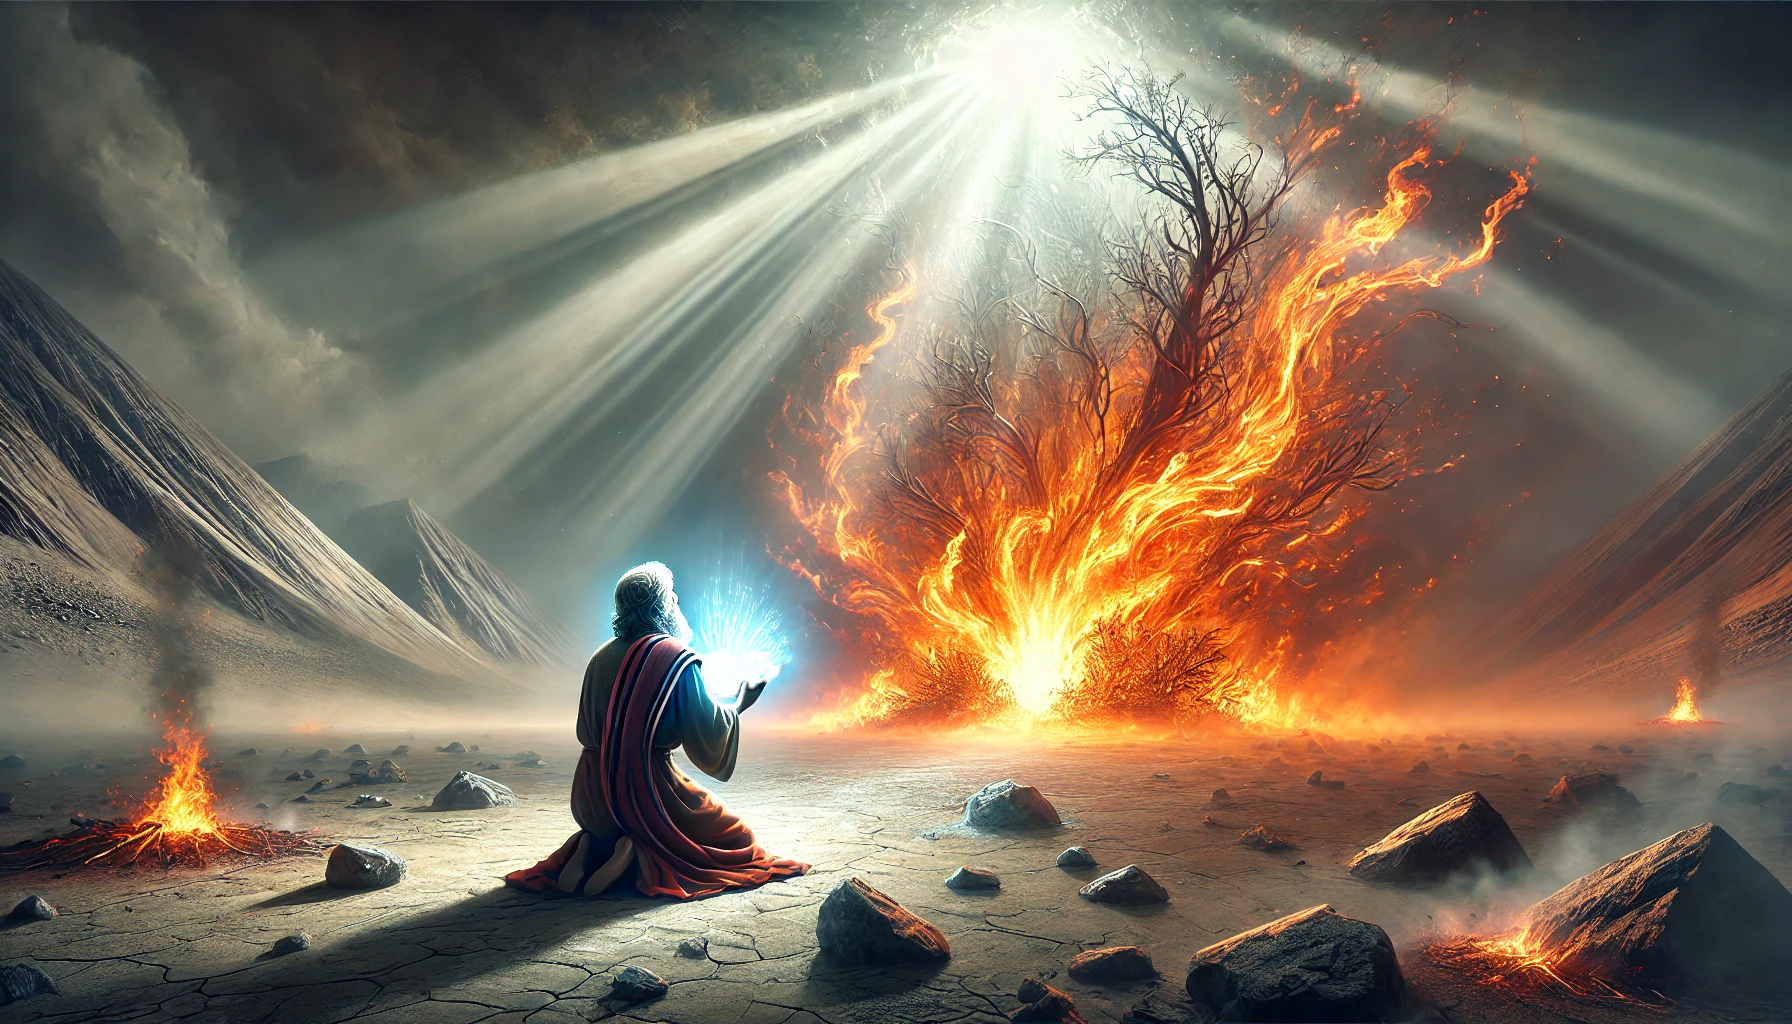
\includegraphics[width=0.99\linewidth]{graficas/exodo}\\
	Moisés ante la zarza ardiente 
	\end{center}



\section*{Capítulo 1}
Aflicción de los israelitas en Egipto  




1:1 Estos son los nombres de los hijos de Israel que entraron en Egipto con Jacob; cada uno entró con su familia:  
1:2 Rubén, Simeón, Leví, Judá,  
1:3 Isacar, Zabulón, Benjamín,  
1:4 Dan, Neftalí, Gad y Aser.  
1:5 Todas las personas que le nacieron a Jacob fueron setenta. Y José estaba en Egipto.  
1:6 Y murió José, y todos sus hermanos, y toda aquella generación.  
1:7 Y los hijos de Israel fructificaron y se multiplicaron, y fueron aumentados y fortalecidos en extremo, y se llenó de ellos la tierra.  
1:8 Entretanto, se levantó sobre Egipto un nuevo rey que no conocía a José; y dijo a su pueblo:  
1:9 He aquí, el pueblo de los hijos de Israel es mayor y más fuerte que nosotros.  
1:10 Ahora, pues, seamos sabios para con él, para que no se multiplique, y acontezca que viniendo guerra, él también se una a nuestros enemigos y pelee contra nosotros, y se vaya de la tierra.  
1:11 Entonces pusieron sobre ellos comisarios de tributos que los molestasen con sus cargas; y edificaron para Faraón las ciudades de almacenaje, Pitón y Ramesés.  
1:12 Pero cuanto más los oprimían, tanto más se multiplicaban y crecían, de manera que los egipcios temían a los hijos de Israel.  
1:13 Y los egipcios hicieron servir a los hijos de Israel con dureza,  
1:14 y amargaron su vida con dura servidumbre, en hacer barro y ladrillo, y en toda labor del campo y en todo su servicio, al cual los obligaban con rigor.  
1:15 Y habló el rey de Egipto a las parteras de las hebreas, una de las cuales se llamaba Sifra, y otra Fúa, y les dijo:  
1:16 Cuando asistáis a las hebreas en sus partos, y veáis el sexo, si es hijo, matadlo; y si es hija, entonces viva.  
1:17 Pero las parteras temieron a Dios, y no hicieron como les mandó el rey de Egipto, sino que preservaron la vida a los niños.  
1:18 Y el rey de Egipto hizo llamar a las parteras y les dijo: ¿Por qué habéis hecho esto, que habéis preservado la vida a los niños?  
1:19 Y las parteras respondieron a Faraón: Porque las mujeres hebreas no son como las egipcias; pues son robustas, y dan a luz antes que la partera venga a ellas.  
1:20 Y Dios hizo bien a las parteras; y el pueblo se multiplicó y se fortaleció en gran manera.  
1:21 Y por haber las parteras temido a Dios, él prosperó sus familias.  
1:22 Entonces Faraón mandó a todo su pueblo, diciendo: Echad al río a todo hijo que nazca, y a toda hija preservad la vida.  
\section*{Capítulo 2}
Nacimiento de Moisés  

2:1 Un varón de la familia de Leví fue y tomó por mujer a una hija de Leví,  
2:2 la que concibió, y dio a luz un hijo; y viéndole que era hermoso, le tuvo escondido tres meses.  
2:3 Pero no pudiendo ocultarle más tiempo, tomó una arquilla de juncos y la calafateó con asfalto y brea, y colocó en ella al niño y lo puso en un carrizal a la orilla del río.  
2:4 Y una hermana suya se puso a lo lejos, para ver lo que le acontecería.  
2:5 Y la hija de Faraón descendió a lavarse al río, y paseándose sus doncellas por la ribera del río, vio ella la arquilla en el carrizal, y envió una criada suya a que la tomase.  
2:6 Y cuando la abrió, vio al niño; y he aquí que el niño lloraba. Y teniendo compasión de él, dijo: De los niños de los hebreos es éste.  
2:7 Entonces su hermana dijo a la hija de Faraón: ¿Iré a llamarte una nodriza de las hebreas, para que te críe este niño?  
2:8 Y la hija de Faraón respondió: Ve. Entonces fue la doncella, y llamó a la madre del niño,  
2:9 a la cual dijo la hija de Faraón: Lleva a este niño y críamelo, y yo te lo pagaré. Y la mujer tomó al niño y lo crió.  
2:10 Y cuando el niño creció, ella lo trajo a la hija de Faraón, la cual lo prohijó, y le puso por nombre Moisés, diciendo: Porque de las aguas lo saqué.  
Moisés huye de Egipto  
2:11 En aquellos días sucedió que crecido ya Moisés, salió a sus hermanos, y los vio en sus duras tareas, y observó a un egipcio que golpeaba a uno de los hebreos, sus hermanos.  
2:12 Entonces miró a todas partes, y viendo que no parecía nadie, mató al egipcio y lo escondió en la arena.  
2:13 Al día siguiente salió y vio a dos hebreos que reñían; entonces dijo al que maltrataba al otro: ¿Por qué golpeas a tu prójimo?  
2:14 Y él respondió: ¿Quién te ha puesto a ti por príncipe y juez sobre nosotros? ¿Piensas matarme como mataste al egipcio? Entonces Moisés tuvo miedo, y dijo: Ciertamente esto ha sido descubierto.  
2:15 Oyendo Faraón acerca de este hecho, procuró matar a Moisés; pero Moisés huyó de delante de Faraón, y habitó en la tierra de Madián. 
2:16 Y estando sentado junto al pozo, siete hijas que tenía el sacerdote de Madián vinieron a sacar agua para llenar las pilas y dar de beber a las ovejas de su padre.  
2:17 Mas los pastores vinieron y las echaron de allí; entonces Moisés se levantó y las defendió, y dio de beber a sus ovejas.  
2:18 Y volviendo ellas a Reuel su padre, él les dijo: ¿Por qué habéis venido hoy tan pronto?  
2:19 Ellas respondieron: Un varón egipcio nos defendió de mano de los pastores, y también nos sacó el agua, y dio de beber a las ovejas.  
2:20 Y dijo a sus hijas: ¿Dónde está? ¿Por qué habéis dejado a ese hombre? Llamadle para que coma.  
2:21 Y Moisés convino en morar con aquel varón; y él dio su hija Séfora por mujer a Moisés.  
2:22 Y ella le dio a luz un hijo; y él le puso por nombre Gersón, porque dijo: Forastero soy en tierra ajena.  
2:23 Aconteció que después de muchos días murió el rey de Egipto, y los hijos de Israel gemían a causa de la servidumbre, y clamaron; y subió a Dios el clamor de ellos con motivo de su servidumbre.  
2:24 Y oyó Dios el gemido de ellos, y se acordó de su pacto con Abraham, Isaac y Jacob.  
2:25 Y miró Dios a los hijos de Israel, y los reconoció Dios.  
\section*{Capítulo 3}
Llamamiento de Moisés 

3:1 Apacentando Moisés las ovejas de Jetro su suegro, sacerdote de Madián, llevó las ovejas a través del desierto, y llegó hasta Horeb, monte de Dios.  
3:2 Y se le apareció el Angel de Jehová en una llama de fuego en medio de una zarza; y él miró, y vio que la zarza ardía en fuego, y la zarza no se consumía.  
3:3 Entonces Moisés dijo: Iré yo ahora y veré esta grande visión, por qué causa la zarza no se quema.  
3:4 Viendo Jehová que él iba a ver, lo llamó Dios de en medio de la zarza, y dijo: ¡Moisés, Moisés! Y él respondió: Heme aquí.  
3:5 Y dijo: No te acerques; quita tu calzado de tus pies, porque el lugar en que tú estás, tierra santa es.  
3:6 Y dijo: Yo soy el Dios de tu padre, Dios de Abraham, Dios de Isaac, y Dios de Jacob. Entonces Moisés cubrió su rostro, porque tuvo miedo de mirar a Dios.  
3:7 Dijo luego Jehová: Bien he visto la aflicción de mi pueblo que está en Egipto, y he oído su clamor a causa de sus exactores; pues he conocido sus angustias,  
3:8 y he descendido para librarlos de mano de los egipcios, y sacarlos de aquella tierra a una tierra buena y ancha, a tierra que fluye leche y miel, a los lugares del cananeo, del heteo, del amorreo, del ferezeo, del heveo y del jebuseo.  
3:9 El clamor, pues, de los hijos de Israel ha venido delante de mí, y también he visto la opresión con que los egipcios los oprimen.  
3:10 Ven, por tanto, ahora, y te enviaré a Faraón, para que saques de Egipto a mi pueblo, los hijos de Israel.  
3:11 Entonces Moisés respondió a Dios: ¿Quién soy yo para que vaya a Faraón, y saque de Egipto a los hijos de Israel?  
3:12 Y él respondió: Ve, porque yo estaré contigo; y esto te será por señal de que yo te he enviado: cuando hayas sacado de Egipto al pueblo, serviréis a Dios sobre este monte.  
3:13 Dijo Moisés a Dios: He aquí que llego yo a los hijos de Israel, y les digo: El Dios de vuestros padres me ha enviado a vosotros. Si ellos me preguntaren: ¿Cuál es su nombre?, ¿qué les responderé?  
3:14 Y respondió Dios a Moisés: YO SOY EL QUE SOY. Y dijo: Así dirás a los hijos de Israel: YO SOY me envió a vosotros.  
3:15 Además dijo Dios a Moisés: Así dirás a los hijos de Israel: Jehová, el Dios de vuestros padres, el Dios de Abraham, Dios de Isaac y Dios de Jacob, me ha enviado a vosotros. Este es mi nombre para siempre; con él se me recordará por todos los siglos.  
3:16 Ve, y reúne a los ancianos de Israel, y diles: Jehová, el Dios de vuestros padres, el Dios de Abraham, de Isaac y de Jacob, me apareció diciendo: En verdad os he visitado, y he visto lo que se os hace en Egipto;  
3:17 y he dicho: Yo os sacaré de la aflicción de Egipto a la tierra del cananeo, del heteo, del amorreo, del ferezeo, del heveo y del jebuseo, a una tierra que fluye leche y miel.  
3:18 Y oirán tu voz; e irás tú, y los ancianos de Israel, al rey de Egipto, y le diréis: Jehová el Dios de los hebreos nos ha encontrado; por tanto, nosotros iremos ahora camino de tres días por el desierto, para que ofrezcamos sacrificios a Jehová nuestro Dios.  
3:19 Mas yo sé que el rey de Egipto no os dejará ir sino por mano fuerte.  
3:20 Pero yo extenderé mi mano, y heriré a Egipto con todas mis maravillas que haré en él, y entonces os dejará ir.  
3:21 Y yo daré a este pueblo gracia en los ojos de los egipcios, para que cuando salgáis, no vayáis con las manos vacías;  
3:22 sino que pedirá cada mujer a su vecina y a su huéspeda alhajas de plata, alhajas de oro, y vestidos, los cuales pondréis sobre vuestros hijos y vuestras hijas; y despojaréis a Egipto. 
\section*{Capítulo 4 }

4:1 Entonces Moisés respondió diciendo: He aquí que ellos no me creerán, ni oirán mi voz; porque dirán: No te ha aparecido Jehová.  
4:2 Y Jehová dijo: ¿Qué es eso que tienes en tu mano? Y él respondió: Una vara.  
4:3 El le dijo: Echala en tierra. Y él la echó en tierra, y se hizo una culebra; y Moisés huía de ella.  
4:4 Entonces dijo Jehová a Moisés: Extiende tu mano, y tómala por la cola. Y él extendió su mano, y la tomó, y se volvió vara en su mano.  
4:5 Por esto creerán que se te ha aparecido Jehová, el Dios de tus padres, el Dios de Abraham, Dios de Isaac y Dios de Jacob.  
4:6 Le dijo además Jehová: Mete ahora tu mano en tu seno. Y él metió la mano en su seno; y cuando la sacó, he aquí que su mano estaba leprosa como la nieve.  
4:7 Y dijo: Vuelve a meter tu mano en tu seno. Y él volvió a meter su mano en su seno; y al sacarla de nuevo del seno, he aquí que se había vuelto como la otra carne.  
4:8 Si aconteciere que no te creyeren ni obedecieren a la voz de la primera señal, creerán a la voz de la postrera.  
4:9 Y si aún no creyeren a estas dos señales, ni oyeren tu voz, tomarás de las aguas del río y las derramarás en tierra; y se cambiarán aquellas aguas que tomarás del río y se harán sangre en la tierra.  
4:10 Entonces dijo Moisés a Jehová: ¡Ay, Señor! nunca he sido hombre de fácil palabra, ni antes, ni desde que tú hablas a tu siervo; porque soy tardo en el habla y torpe de lengua.  
4:11 Y Jehová le respondió: ¿Quién dio la boca al hombre? ¿o quién hizo al mudo y al sordo, al que ve y al ciego? ¿No soy yo Jehová?  
4:12 Ahora pues, ve, y yo estaré con tu boca, y te enseñaré lo que hayas de hablar.  
4:13 Y él dijo: ¡Ay, Señor! envía, te ruego, por medio del que debes enviar.  
4:14 Entonces Jehová se enojó contra Moisés, y dijo: ¿No conozco yo a tu hermano Aarón, levita, y que él habla bien? Y he aquí que él saldrá a recibirte, y al verte se alegrará en su corazón.  
4:15 Tú hablarás a él, y pondrás en su boca las palabras, y yo estaré con tu boca y con la suya, y os enseñaré lo que hayáis de hacer.  
4:16 Y él hablará por ti al pueblo; él te será a ti en lugar de boca, y tú serás para él en lugar de Dios.  
4:17 Y tomarás en tu mano esta vara, con la cual harás las señales. 
Moisés vuelve a Egipto  
4:18 Así se fue Moisés, y volviendo a su suegro Jetro, le dijo: Iré ahora, y volveré a mis hermanos que están en Egipto, para ver si aún viven. Y Jetro dijo a Moisés: Ve en paz.  
4:19 Dijo también Jehová a Moisés en Madián: Ve y vuélvete a Egipto, porque han muerto todos los que procuraban tu muerte.  
4:20 Entonces Moisés tomó su mujer y sus hijos, y los puso sobre un asno, y volvió a tierra de Egipto. Tomó también Moisés la vara de Dios en su mano.  
4:21 Y dijo Jehová a Moisés: Cuando hayas vuelto a Egipto, mira que hagas delante de Faraón todas las maravillas que he puesto en tu mano; pero yo endureceré su corazón, de modo que no dejará ir al pueblo.  
4:22 Y dirás a Faraón: Jehová ha dicho así: Israel es mi hijo, mi primogénito.  
4:23 Ya te he dicho que dejes ir a mi hijo, para que me sirva, mas no has querido dejarlo ir; he aquí yo voy a matar a tu hijo, tu primogénito. 
4:24 Y aconteció en el camino, que en una posada Jehová le salió al encuentro, y quiso matarlo.  
4:25 Entonces Séfora tomó un pedernal afilado y cortó el prepucio de su hijo, y lo echó a sus pies, diciendo: A la verdad tú me eres un esposo de sangre.  
4:26 Así le dejó luego ir. Y ella dijo: Esposo de sangre, a causa de la circuncisión.  
4:27 Y Jehová dijo a Aarón: Ve a recibir a Moisés al desierto. Y él fue, y lo encontró en el monte de Dios, y le besó.  
4:28 Entonces contó Moisés a Aarón todas las palabras de Jehová que le enviaba, y todas las señales que le había dado.  
4:29 Y fueron Moisés y Aarón, y reunieron a todos los ancianos de los hijos de Israel.  
4:30 Y habló Aarón acerca de todas las cosas que Jehová había dicho a Moisés, e hizo las señales delante de los ojos del pueblo.  
4:31 Y el pueblo creyó; y oyendo que Jehová había visitado a los hijos de Israel, y que había visto su aflicción, se inclinaron y adoraron.  
\section*{Capítulo 5}
Moisés y Aarón ante Faraón  

5:1 Después Moisés y Aarón entraron a la presencia de Faraón y le dijeron: Jehová el Dios de Israel dice así: Deja ir a mi pueblo a celebrarme fiesta en el desierto.  
5:2 Y Faraón respondió: ¿Quién es Jehová, para que yo oiga su voz y deje ir a Israel? Yo no conozco a Jehová, ni tampoco dejaré ir a Israel.  
5:3 Y ellos dijeron: El Dios de los hebreos nos ha encontrado; iremos, pues, ahora, camino de tres días por el desierto, y ofreceremos sacrificios a Jehová nuestro Dios, para que no venga sobre nosotros con peste o con espada.  
5:4 Entonces el rey de Egipto les dijo: Moisés y Aarón, ¿por qué hacéis cesar al pueblo de su trabajo? Volved a vuestras tareas.  
5:5 Dijo también Faraón: He aquí el pueblo de la tierra es ahora mucho, y vosotros les hacéis cesar de sus tareas.  
5:6 Y mandó Faraón aquel mismo día a los cuadrilleros del pueblo que lo tenían a su cargo, y a sus capataces, diciendo:  
5:7 De aquí en adelante no daréis paja al pueblo para hacer ladrillo, como hasta ahora; vayan ellos y recojan por sí mismos la paja.  
5:8 Y les impondréis la misma tarea de ladrillo que hacían antes, y no les disminuiréis nada; porque están ociosos, por eso levantan la voz diciendo: Vamos y ofrezcamos sacrificios a nuestro Dios.  
5:9 Agrávese la servidumbre sobre ellos, para que se ocupen en ella, y no atiendan a palabras mentirosas.  
5:10 Y saliendo los cuadrilleros del pueblo y sus capataces, hablaron al pueblo, diciendo: Así ha dicho Faraón: Yo no os doy paja.  
5:11 Id vosotros y recoged la paja donde la halléis; pero nada se disminuirá de vuestra tarea.  
5:12 Entonces el pueblo se esparció por toda la tierra de Egipto para recoger rastrojo en lugar de paja.  
5:13 Y los cuadrilleros los apremiaban, diciendo: Acabad vuestra obra, la tarea de cada día en su día, como cuando se os daba paja.  
5:14 Y azotaban a los capataces de los hijos de Israel que los cuadrilleros de Faraón habían puesto sobre ellos, diciendo: ¿Por qué no habéis cumplido vuestra tarea de ladrillo ni ayer ni hoy, como antes?  
5:15 Y los capataces de los hijos de Israel vinieron a Faraón y se quejaron a él, diciendo: ¿Por qué lo haces así con tus siervos?  
5:16 No se da paja a tus siervos, y con todo nos dicen: Haced el ladrillo. Y he aquí tus siervos son azotados, y el pueblo tuyo es el culpable.  
5:17 Y él respondió: Estáis ociosos, sí, ociosos, y por eso decís: Vamos y ofrezcamos sacrificios a Jehová.  
5:18 Id pues, ahora, y trabajad. No se os dará paja, y habéis de entregar la misma tarea de ladrillo.  
5:19 Entonces los capataces de los hijos de Israel se vieron en aflicción, al decírseles: No se disminuirá nada de vuestro ladrillo, de la tarea de cada día.  
5:20 Y encontrando a Moisés y a Aarón, que estaban a la vista de ellos cuando salían de la presencia de Faraón,  
5:21 les dijeron: Mire Jehová sobre vosotros, y juzgue; pues nos habéis hecho abominables delante de Faraón y de sus siervos, poniéndoles la espada en la mano para que nos maten.  
Jehová comisiona a Moisés y a Aarón 
5:22 Entonces Moisés se volvió a Jehová, y dijo: Señor, ¿por qué afliges a este pueblo? ¿Para qué me enviaste?  
5:23 Porque desde que yo vine a Faraón para hablarle en tu nombre, ha afligido a este pueblo; y tú no has librado a tu pueblo.  
\section*{Capítulo 6 }

6:1 Jehová respondió a Moisés: Ahora verás lo que yo haré a Faraón; porque con mano fuerte los dejará ir, y con mano fuerte los echará de su tierra.  
6:2 Habló todavía Dios a Moisés, y le dijo: Yo soy JEHOVÁ.  
6:3 Y aparecí a Abraham, a Isaac y a Jacob como Dios Omnipotente,  mas en mi nombre JEHOVÁ no me di a conocer a ellos.  
6:4 También establecí mi pacto con ellos, de darles la tierra de Canaán, la tierra en que fueron forasteros, y en la cual habitaron.  
6:5 Asimismo yo he oído el gemido de los hijos de Israel, a quienes hacen servir los egipcios, y me he acordado de mi pacto.  
6:6 Por tanto, dirás a los hijos de Israel: Yo soy JEHOVÁ; y yo os sacaré de debajo de las tareas pesadas de Egipto, y os libraré de su servidumbre, y os redimiré con brazo extendido, y con juicios grandes;  
6:7 y os tomaré por mi pueblo y seré vuestro Dios; y vosotros sabréis que yo soy Jehová vuestro Dios, que os sacó de debajo de las tareas pesadas de Egipto.  
6:8 Y os meteré en la tierra por la cual alcé mi mano jurando que la daría a Abraham, a Isaac y a Jacob; y yo os la daré por heredad. Yo JEHOVÁ.  
6:9 De esta manera habló Moisés a los hijos de Israel; pero ellos no escuchaban a Moisés a causa de la congoja de espíritu, y de la dura servidumbre.  
6:10 Y habló Jehová a Moisés, diciendo:  
6:11 Entra y habla a Faraón rey de Egipto, que deje ir de su tierra a los hijos de Israel.  
6:12 Y respondió Moisés delante de Jehová: He aquí, los hijos de Israel no me escuchan; ¿cómo, pues, me escuchará Faraón, siendo yo torpe de labios?  
6:13 Entonces Jehová habló a Moisés y a Aarón y les dio mandamiento para los hijos de Israel, y para Faraón rey de Egipto, para que sacasen a los hijos de Israel de la tierra de Egipto.  
6:14 Estos son los jefes de las familias de sus padres: Los hijos de Rubén, el primogénito de Israel: Hanoc, Falú, Hezrón y Carmi; estas son las familias de Rubén.  
6:15 Los hijos de Simeón: Jemuel, Jamín, Ohad, Jaquín, Zohar, y Saúl hijo de una cananea. Estas son las familias de Simeón.  
6:16 Estos son los nombres de los hijos de Leví por sus linajes: Gersón, Coat y Merari. Y los años de la vida de Leví fueron ciento treinta y siete años.  
6:17 Los hijos de Gersón: Libni y Simei, por sus familias.  
6:18 Y los hijos de Coat: Amram, Izhar, Hebrón y Uziel. Y los años de la vida de Coat fueron ciento treinta y tres años.  
6:19 Y los hijos de Merari: Mahli y Musi. Estas son las familas de Leví por sus linajes. 
6:20 Y Amram tomó por mujer a Jocabed su tía, la cual dio a luz a Aarón y a Moisés. Y los años de la vida de Amram fueron ciento treinta y siete años.  
6:21 Los hijos de Izhar: Coré, Nefeg y Zicri.  
6:22 Y los hijos de Uziel: Misael, Elzafán y Sitri.  
6:23 Y tomó Aarón por mujer a Elisabet hija de Aminadab, hermana de Naasón; la cual dio a luz a Nadab, Abiú, Eleazar e Itamar.  
6:24 Los hijos de Coré: Asir, Elcana y Abiasaf. Estas son las familias de los coreítas.  
6:25 Y Eleazar hijo de Aarón tomó para sí mujer de las hijas de Futiel, la cual dio a luz a Finees. Y estos son los jefes de los padres de los levitas por sus familias.  
6:26 Este es aquel Aarón y aquel Moisés, a los cuales Jehová dijo: Sacad a los hijos de Israel de la tierra de Egipto por sus ejércitos.  
6:27 Estos son los que hablaron a Faraón rey de Egipto, para sacar de Egipto a los hijos de Israel. Moisés y Aarón fueron éstos.  
6:28 Cuando Jehová habló a Moisés en la tierra de Egipto,  
6:29 entonces Jehová habló a Moisés, diciendo: Yo soy JEHOVÁ; di a Faraón rey de Egipto todas las cosas que yo te digo a ti.  
6:30 Y Moisés respondió delante de Jehová: He aquí, yo soy torpe de labios; ¿cómo, pues, me ha de oír Faraón?  
\section*{Capítulo 7 }

7:1 Jehová dijo a Moisés: Mira, yo te he constituido dios para Faraón, y tu hermano Aarón será tu profeta. 
7:2 Tú dirás todas las cosas que yo te mande, y Aarón tu hermano hablará a Faraón, para que deje ir de su tierra a los hijos de Israel.  
7:3 Y yo endureceré el corazón de Faraón, y multiplicaré en la tierra de Egipto mis señales y mis maravillas.  
7:4 Y Faraón no os oirá; mas yo pondré mi mano sobre Egipto, y sacaré a mis ejércitos, mi pueblo, los hijos de Israel, de la tierra de Egipto, con grandes juicios.  
7:5 Y sabrán los egipcios que yo soy Jehová, cuando extienda mi mano sobre Egipto, y saque a los hijos de Israel de en medio de ellos.  
7:6 E hizo Moisés y Aarón como Jehová les mandó; así lo hicieron.  
7:7 Era Moisés de edad de ochenta años, y Aarón de edad de ochenta y tres, cuando hablaron a Faraón.  
La vara de Aarón  
7:8 Habló Jehová a Moisés y a Aarón, diciendo:  
7:9 Si Faraón os respondiere diciendo: Mostrad milagro; dirás a Aarón: Toma tu vara, y échala delante de Faraón, para que se haga culebra.  
7:10 Vinieron, pues, Moisés y Aarón a Faraón, e hicieron como Jehová lo había mandado. Y echó Aarón su vara delante de Faraón y de sus siervos, y se hizo culebra.  
7:11 Entonces llamó también Faraón sabios y hechiceros, e hicieron también lo mismo los hechiceros de Egipto con sus encantamientos;  
7:12 pues echó cada uno su vara, las cuales se volvieron culebras; mas la vara de Aarón devoró las varas de ellos.  
7:13 Y el corazón de Faraón se endureció, y no los escuchó, como Jehová lo había dicho.  
La plaga de sangre  
7:14 Entonces Jehová dijo a Moisés: El corazón de Faraón está endurecido, y no quiere dejar ir al pueblo.  
7:15 Ve por la mañana a Faraón, he aquí que él sale al río; y tú ponte a la ribera delante de él, y toma en tu mano la vara que se volvió culebra,  
7:16 y dile: Jehová el Dios de los hebreos me ha enviado a ti, diciendo: Deja ir a mi pueblo, para que me sirva en el desierto; y he aquí que hasta ahora no has querido oír.  
7:17 Así ha dicho Jehová: En esto conocerás que yo soy Jehová: he aquí, yo golpearé con la vara que tengo en mi mano el agua que está en el río, y se convertirá en sangre.  
7:18 Y los peces que hay en el río morirán, y hederá el río, y los egipcios tendrán asco de beber el agua del río.  
7:19 Y Jehová dijo a Moisés: Di a Aarón: Toma tu vara, y extiende tu mano sobre las aguas de Egipto, sobre sus ríos, sobre sus arroyos y sobre sus estanques, y sobre todos sus depósitos de aguas, para que se conviertan en sangre, y haya sangre por toda la región de Egipto, así en los vasos de madera como en los de piedra.  
7:20 Y Moisés y Aarón hicieron como Jehová lo mandó; y alzando la vara golpeó las aguas que había en el río, en presencia de Faraón y de sus siervos; y todas las aguas que había en el río se convirtieron en sangre.  
7:21 Asimismo los peces que había en el río murieron; y el río se corrompió, tanto que los egipcios no podían beber de él. Y hubo sangre por toda la tierra de Egipto.  
7:22 Y los hechiceros de Egipto hicieron lo mismo con sus encantamientos; y el corazón de Faraón se endureció, y no los escuchó; como Jehová lo había dicho.  
7:23 Y Faraón se volvió y fue a su casa, y no dio atención tampoco a esto. 
7:24 Y en todo Egipto hicieron pozos alrededor del río para beber, porque no podían beber de las aguas del río.  
7:25 Y se cumplieron siete días después que Jehová hirió el río.  
\section*{Capítulo 8}
La plaga de ranas 

8:1 Entonces Jehová dijo a Moisés: Entra a la presencia de Faraón y dile: Jehová ha dicho así: Deja ir a mi pueblo, para que me sirva.  
8:2 Y si no lo quisieres dejar ir, he aquí yo castigaré con ranas todos tus territorios.  
8:3 Y el río criará ranas, las cuales subirán y entrarán en tu casa, en la cámara donde duermes, y sobre tu cama, y en las casas de tus siervos, en tu pueblo, en tus hornos y en tus artesas.  
8:4 Y las ranas subirán sobre ti, sobre tu pueblo, y sobre todos tus siervos.  
8:5 Y Jehová dijo a Moisés: Di a Aarón: Extiende tu mano con tu vara sobre los ríos, arroyos y estanques, para que haga subir ranas sobre la tierra de Egipto.  
8:6 Entonces Aarón extendió su mano sobre las aguas de Egipto, y subieron ranas que cubrieron la tierra de Egipto.  
8:7 Y los hechiceros hicieron lo mismo con sus encantamientos, e hicieron venir ranas sobre la tierra de Egipto.  
8:8 Entonces Faraón llamó a Moisés y a Aarón, y les dijo: Orad a Jehová para que quite las ranas de mí y de mi pueblo, y dejaré ir a tu pueblo para que ofrezca sacrificios a Jehová.  
8:9 Y dijo Moisés a Faraón: Dígnate indicarme cuándo debo orar por ti, por tus siervos y por tu pueblo, para que las ranas sean quitadas de ti y de tus casas, y que solamente queden en el río.  
8:10 Y él dijo: Mañana. Y Moisés respondió: Se hará conforme a tu palabra, para que conozcas que no hay como Jehová nuestro Dios.  
8:11 Y las ranas se irán de ti, y de tus casas, de tus siervos y de tu pueblo, y solamente quedarán en el río.  
8:12 Entonces salieron Moisés y Aarón de la presencia de Faraón. Y clamó Moisés a Jehová tocante a las ranas que había mandado a Faraón.  
8:13 E hizo Jehová conforme a la palabra de Moisés, y murieron las ranas de las casas, de los cortijos y de los campos.  
8:14 Y las juntaron en montones, y apestaba la tierra.  
8:15 Pero viendo Faraón que le habían dado reposo, endureció su corazón y no los escuchó, como Jehová lo había dicho.  
La plaga de piojos  
8:16 Entonces Jehová dijo a Moisés: Di a Aarón: Extiende tu vara y golpea el polvo de la tierra, para que se vuelva piojos por todo el país de Egipto.  
8:17 Y ellos lo hicieron así; y Aarón extendió su mano con su vara, y golpeó el polvo de la tierra, el cual se volvió piojos, así en los hombres como en las bestias; todo el polvo de la tierra se volvió piojos en todo el país de Egipto.  
8:18 Y los hechiceros hicieron así también, para sacar piojos con sus encantamientos; pero no pudieron. Y hubo piojos tanto en los hombres como en las bestias.  
8:19 Entonces los hechiceros dijeron a Faraón: Dedo de Dios es éste. Mas el corazón de Faraón se endureció, y no los escuchó, como Jehová lo había dicho.  
La plaga de moscas  
8:20 Jehová dijo a Moisés: Levántate de mañana y ponte delante de Faraón, he aquí él sale al río; y dile: Jehová ha dicho así: Deja ir a mi pueblo, para que me sirva.  
8:21 Porque si no dejas ir a mi pueblo, he aquí yo enviaré sobre ti, sobre tus siervos, sobre tu pueblo y sobre tus casas toda clase de moscas; y las casas de los egipcios se llenarán de toda clase de moscas, y asimismo la tierra donde ellos estén.  
8:22 Y aquel día yo apartaré la tierra de Gosén, en la cual habita mi pueblo, para que ninguna clase de moscas haya en ella, a fin de que sepas que yo soy Jehová en medio de la tierra.  
8:23 Y yo pondré redención entre mi pueblo y el tuyo. Mañana será esta señal.  
8:24 Y Jehová lo hizo así, y vino toda clase de moscas molestísimas sobre la casa de Faraón, sobre las casas de sus siervos, y sobre todo el país de Egipto; y la tierra fue corrompida a causa de ellas.  
8:25 Entonces Faraón llamó a Moisés y a Aarón, y les dijo: Andad, ofreced sacrificio a vuestro Dios en la tierra.  
8:26 Y Moisés respondió: No conviene que hagamos así, porque ofreceríamos a Jehová nuestro Dios la abominación de los egipcios. He aquí, si sacrificáramos la abominación de los egipcios delante de ellos, ¿no nos apedrearían?  
8:27 Camino de tres días iremos por el desierto, y ofreceremos sacrificios a Jehová nuestro Dios, como él nos dirá.  
8:28 Dijo Faraón: Yo os dejaré ir para que ofrezcáis sacrificios a Jehová vuestro Dios en el desierto, con tal que no vayáis más lejos; orad por mí.  
8:29 Y respondió Moisés: He aquí, al salir yo de tu presencia, rogaré a Jehová que las diversas clases de moscas se vayan de Faraón, y de sus siervos, y de su pueblo mañana; con tal que Faraón no falte más, no dejando ir al pueblo a dar sacrificio a Jehová.  
8:30 Entonces Moisés salió de la presencia de Faraón, y oró a Jehová.  
8:31 Y Jehová hizo conforme a la palabra de Moisés, y quitó todas aquellas moscas de Faraón, de sus siervos y de su pueblo, sin que quedara una.  
8:32 Mas Faraón endureció aun esta vez su corazón, y no dejó ir al pueblo.  
\section*{Capítulo 9}
La plaga en el ganado  

9:1 Entonces Jehová dijo a Moisés: Entra a la presencia de Faraón, y dile: Jehová, el Dios de los hebreos, dice así: Deja ir a mi pueblo, para que me sirva.  
9:2 Porque si no lo quieres dejar ir, y lo detienes aún,  
9:3 he aquí la mano de Jehová estará sobre tus ganados que están en el campo, caballos, asnos, camellos, vacas y ovejas, con plaga gravísima.  
9:4 Y Jehová hará separación entre los ganados de Israel y los de Egipto, de modo que nada muera de todo lo de los hijos de Israel.  
9:5 Y Jehová fijó plazo, diciendo: Mañana hará Jehová esta cosa en la tierra.  
9:6 Al día siguiente Jehová hizo aquello, y murió todo el ganado de Egipto; mas del ganado de los hijos de Israel no murió uno.  
9:7 Entonces Faraón envió, y he aquí que del ganado de los hijos de Israel no había muerto uno. Mas el corazón de Faraón se endureció, y no dejó ir al pueblo.  
La plaga de úlceras  
9:8 Y Jehová dijo a Moisés y a Aarón: Tomad puñados de ceniza de un horno, y la esparcirá Moisés hacia el cielo delante de Faraón;  
9:9 y vendrá a ser polvo sobre toda la tierra de Egipto, y producirá sarpullido con úlceras en los hombres y en las bestias, por todo el país de Egipto.  
9:10 Y tomaron ceniza del horno, y se pusieron delante de Faraón, y la esparció Moisés hacia el cielo; y hubo sarpullido que produjo úlceras tanto en los hombres como en las bestias.  
9:11 Y los hechiceros no podían estar delante de Moisés a causa del sarpullido, porque hubo sarpullido en los hechiceros y en todos los egipcios.  
9:12 Pero Jehová endureció el corazón de Faraón, y no los oyó, como Jehová lo había dicho a Moisés.  
La plaga de granizo  
9:13 Entonces Jehová dijo a Moisés: Levántate de mañana, y ponte delante de Faraón, y dile: Jehová, el Dios de los hebreos, dice así: Deja ir a mi pueblo, para que me sirva.  
9:14 Porque yo enviaré esta vez todas mis plagas a tu corazón, sobre tus siervos y sobre tu pueblo, para que entiendas que no hay otro como yo en toda la tierra.  
9:15 Porque ahora yo extenderé mi mano para herirte a ti y a tu pueblo de plaga, y serás quitado de la tierra.  
9:16 Y a la verdad yo te he puesto para mostrar en ti mi poder, y para que mi nombre sea anunciado en toda la tierra.  
9:17 ¿Todavía te ensoberbeces contra mi pueblo, para no dejarlos ir?  
9:18 He aquí que mañana a estas horas yo haré llover granizo muy pesado, cual nunca hubo en Egipto, desde el día que se fundó hasta ahora.  
9:19 Envía, pues, a recoger tu ganado, y todo lo que tienes en el campo; porque todo hombre o animal que se halle en el campo, y no sea recogido a casa, el granizo caerá sobre él, y morirá.  
9:20 De los siervos de Faraón, el que tuvo temor de la palabra de Jehová hizo huir sus criados y su ganado a casa;  
9:21 mas el que no puso en su corazón la palabra de Jehová, dejó sus criados y sus ganados en el campo.  
9:22 Y Jehová dijo a Moisés: Extiende tu mano hacia el cielo, para que venga granizo en toda la tierra de Egipto sobre los hombres, y sobre las bestias, y sobre toda la hierba del campo en el país de Egipto.  
9:23 Y Moisés extendió su vara hacia el cielo, y Jehová hizo tronar y granizar, y el fuego se descargó sobre la tierra; y Jehová hizo llover granizo sobre la tierra de Egipto.  
9:24 Hubo, pues, granizo, y fuego mezclado con el granizo, tan grande, cual nunca hubo en toda la tierra de Egipto desde que fue habitada.  
9:25 Y aquel granizo hirió en toda la tierra de Egipto todo lo que estaba en el campo, así hombres como bestias; asimismo destrozó el granizo toda la hierba del campo, y desgajó todos los árboles del país.  
9:26 Solamente en la tierra de Gosén, donde estaban los hijos de Israel, no hubo granizo. 
9:27 Entonces Faraón envió a llamar a Moisés y a Aarón, y les dijo: He pecado esta vez; Jehová es justo, y yo y mi pueblo impíos.  
9:28 Orad a Jehová para que cesen los truenos de Dios y el granizo, y yo os dejaré ir, y no os detendréis más.  
9:29 Y le respondió Moisés: Tan pronto salga yo de la ciudad, extenderé mis manos a Jehová, y los truenos cesarán, y no habrá más granizo; para que sepas que de Jehová es la tierra.  
9:30 Pero yo sé que ni tú ni tus siervos temeréis todavía la presencia de Jehová Dios.  
9:31 El lino, pues, y la cebada fueron destrozados, porque la cebada estaba ya espigada, y el lino en caña.  
9:32 Mas el trigo y el centeno no fueron destrozados, porque eran tardíos.  
9:33 Y salido Moisés de la presencia de Faraón, fuera de la ciudad, extendió sus manos a Jehová, y cesaron los truenos y el granizo, y la lluvia no cayó más sobre la tierra.  
9:34 Y viendo Faraón que la lluvia había cesado, y el granizo y los truenos, se obstinó en pecar, y endurecieron su corazón él y sus siervos.  
9:35 Y el corazón de Faraón se endureció, y no dejó ir a los hijos de Israel, como Jehová lo había dicho por medio de Moisés.  
\section*{Capítulo 10 }
La plaga de langostas 

10:1 Jehová dijo a Moisés: Entra a la presencia de Faraón; porque yo he endurecido su corazón, y el corazón de sus siervos, para mostrar entre ellos estas mis señales,  
10:2 y para que cuentes a tus hijos y a tus nietos las cosas que yo hice en Egipto, y mis señales que hice entre ellos; para que sepáis que yo soy Jehová.  
10:3 Entonces vinieron Moisés y Aarón a Faraón, y le dijeron: Jehová el Dios de los hebreos ha dicho así: ¿Hasta cuándo no querrás humillarte delante de mí? Deja ir a mi pueblo, para que me sirva.  
10:4 Y si aún rehúsas dejarlo ir, he aquí que mañana yo traeré sobre tu territorio la langosta,  
10:5 la cual cubrirá la faz de la tierra, de modo que no pueda verse la tierra; y ella comerá lo que escapó, lo que os quedó del granizo; comerá asimismo todo árbol que os fructifica en el campo.  
10:6 Y llenará tus casas, y las casas de todos tus siervos, y las casas de todos los egipcios, cual nunca vieron tus padres ni tus abuelos, desde que ellos fueron sobre la tierra hasta hoy. Y se volvió y salió de delante de Faraón.  
10:7 Entonces los siervos de Faraón le dijeron: ¿Hasta cuándo será este hombre un lazo para nosotros? Deja ir a estos hombres, para que sirvan a Jehová su Dios. ¿Acaso no sabes todavía que Egipto está ya destruido?  
10:8 Y Moisés y Aarón volvieron a ser llamados ante Faraón, el cual les dijo: Andad, servid a Jehová vuestro Dios. ¿Quiénes son los que han de ir?  
10:9 Moisés respondió: Hemos de ir con nuestros niños y con nuestros viejos, con nuestros hijos y con nuestras hijas; con nuestras ovejas y con nuestras vacas hemos de ir; porque es nuestra fiesta solemne para Jehová.  
10:10 Y él les dijo: ¡Así sea Jehová con vosotros! ¿Cómo os voy a dejar ir a vosotros y a vuestros niños? ¡Mirad cómo el mal está delante de vuestro rostro! 
10:11 No será así; id ahora vosotros los varones, y servid a Jehová, pues esto es lo que vosotros pedisteis. Y los echaron de la presencia de Faraón.  
10:12 Entonces Jehová dijo a Moisés: Extiende tu mano sobre la tierra de Egipto para traer la langosta, a fin de que suba sobre el país de Egipto, y consuma todo lo que el granizo dejó.  
10:13 Y extendió Moisés su vara sobre la tierra de Egipto, y Jehová trajo un viento oriental sobre el país todo aquel día y toda aquella noche; y al venir la mañana el viento oriental trajo la langosta.  
10:14 Y subió la langosta sobre toda la tierra de Egipto, y se asentó en todo el país de Egipto en tan gran cantidad como no la hubo antes ni la habrá después;  
10:15 y cubrió la faz de todo el país, y oscureció la tierra; y consumió toda la hierba de la tierra, y todo el fruto de los árboles que había dejado el granizo; no quedó cosa verde en árboles ni en hierba del campo, en toda la tierra de Egipto.  
10:16 Entonces Faraón se apresuró a llamar a Moisés y a Aarón, y dijo: He pecado contra Jehová vuestro Dios, y contra vosotros.  
10:17 Mas os ruego ahora que perdonéis mi pecado solamente esta vez, y que oréis a Jehová vuestro Dios que quite de mí al menos esta plaga mortal.  
10:18 Y salió Moisés de delante de Faraón, y oró a Jehová.  
10:19 Entonces Jehová trajo un fortísimo viento occidental, y quitó la langosta y la arrojó en el Mar Rojo; ni una langosta quedó en todo el país de Egipto.  
10:20 Pero Jehová endureció el corazón de Faraón, y éste no dejó ir a los hijos de Israel.  
La plaga de tinieblas  
10:21 Jehová dijo a Moisés: Extiende tu mano hacia el cielo, para que haya tinieblas  sobre la tierra de Egipto, tanto que cualquiera las palpe.  
10:22 Y extendió Moisés su mano hacia el cielo, y hubo densas tinieblas sobre toda la tierra de Egipto, por tres días.  
10:23 Ninguno vio a su prójimo, ni nadie se levantó de su lugar en tres días; mas todos los hijos de Israel tenían luz en sus habitaciones.  
10:24 Entonces Faraón hizo llamar a Moisés, y dijo: Id, servid a Jehová; solamente queden vuestras ovejas y vuestras vacas; vayan también vuestros niños con vosotros. 
10:25 Y Moisés respondió: Tú también nos darás sacrificios y holocaustos que sacrifiquemos para Jehová nuestro Dios.  
10:26 Nuestros ganados irán también con nosotros; no quedará ni una pezuña; porque de ellos hemos de tomar para servir a Jehová nuestro Dios, y no sabemos con qué hemos de servir a Jehová hasta que lleguemos allá.  
10:27 Pero Jehová endureció el corazón de Faraón, y no quiso dejarlos ir.  
10:28 Y le dijo Faraón: Retírate de mí; guárdate que no veas más mi rostro, porque en cualquier día que vieres mi rostro, morirás.  
10:29 Y Moisés respondió: Bien has dicho; no veré más tu rostro.  
\section*{Capítulo 11}
Anunciada la muerte de los primogénitos 

11:1 Jehová dijo a Moisés: Una plaga traeré aún sobre Faraón y sobre Egipto, después de la cual él os dejará ir de aquí; y seguramente os echará de aquí del todo.  
11:2 Habla ahora al pueblo, y que cada uno pida a su vecino, y cada una a su vecina, alhajas de plata y de oro.  
11:3 Y Jehová dio gracia al pueblo en los ojos de los egipcios. También Moisés era tenido por gran varón en la tierra de Egipto, a los ojos de los siervos de Faraón, y a los ojos del pueblo.  
11:4 Dijo, pues, Moisés: Jehová ha dicho así: A la medianoche yo saldré por en medio de Egipto,  
11:5 y morirá todo primogénito en tierra de Egipto, desde el primogénito de Faraón que se sienta en su trono, hasta el primogénito de la sierva que está tras el molino, y todo primogénito de las bestias.  
11:6 Y habrá gran clamor por toda la tierra de Egipto, cual nunca hubo, ni jamás habrá.  
11:7 Pero contra todos los hijos de Israel, desde el hombre hasta la bestia, ni un perro moverá su lengua, para que sepáis que Jehová hace diferencia entre los egipcios y los israelitas.  
11:8 Y descenderán a mí todos estos tus siervos, e inclinados delante de mí dirán: Vete, tú y todo el pueblo que está debajo de ti; y después de esto yo saldré. Y salió muy enojado de la presencia de Faraón.  
11:9 Y Jehová dijo a Moisés: Faraón no os oirá, para que mis maravillas se multipliquen en la tierra de Egipto.  
11:10 Y Moisés y Aarón hicieron todos estos prodigios delante de Faraón; pues Jehová había endurecido el corazón de Faraón, y no envió a los hijos de Israel fuera de su país.  
\section*{Capítulo 12}
La Pascua  

12:1 Habló Jehová a Moisés y a Aarón en la tierra de Egipto, diciendo:  
12:2 Este mes os será principio de los meses; para vosotros será éste el primero en los meses del año.  
12:3 Hablad a toda la congregación de Israel, diciendo: En el diez de este mes tómese cada uno un cordero según las familias de los padres, un cordero por familia.  
12:4 Mas si la familia fuere tan pequeña que no baste para comer el cordero, entonces él y su vecino inmediato a su casa tomarán uno según el número de las personas; conforme al comer de cada hombre, haréis la cuenta sobre el cordero.  
12:5 El animal será sin defecto, macho de un año; lo tomaréis de las ovejas o de las cabras.  
12:6 Y lo guardaréis hasta el día catorce de este mes, y lo inmolará toda la congregación del pueblo de Israel entre las dos tardes.  
12:7 Y tomarán de la sangre, y la pondrán en los dos postes y en el dintel de las casas en que lo han de comer.  
12:8 Y aquella noche comerán la carne asada al fuego, y panes sin levadura; con hierbas amargas lo comerán.  
12:9 Ninguna cosa comeréis de él cruda, ni cocida en agua, sino asada al fuego; su cabeza con sus pies y sus entrañas.  
12:10 Ninguna cosa dejaréis de él hasta la mañana; y lo que quedare hasta la mañana, lo quemaréis en el fuego.  
12:11 Y lo comeréis así: ceñidos vuestros lomos, vuestro calzado en vuestros pies, y vuestro bordón en vuestra mano; y lo comeréis apresuradamente; es la Pascua de Jehová.  
12:12 Pues yo pasaré aquella noche por la tierra de Egipto, y heriré a todo primogénito en la tierra de Egipto, así de los hombres como de las bestias; y ejecutaré mis juicios en todos los dioses de Egipto. Yo Jehová. 
12:13 Y la sangre os será por señal en las casas donde vosotros estéis; y veré la sangre y pasaré de vosotros, y no habrá en vosotros plaga de mortandad cuando hiera la tierra de Egipto.  
12:14 Y este día os será en memoria, y lo celebraréis como fiesta solemne para Jehová durante vuestras generaciones; por estatuto perpetuo lo celebraréis.  
12:15 Siete días comeréis panes sin levadura; y así el primer día haréis que no haya levadura en vuestras casas; porque cualquiera que comiere leudado desde el primer día hasta el séptimo, será cortado de Israel.  
12:16 El primer día habrá santa convocación, y asimismo en el séptimo día tendréis una santa convocación; ninguna obra se hará en ellos, excepto solamente que preparéis lo que cada cual haya de comer.  
12:17 Y guardaréis la fiesta de los panes sin levadura,  porque en este mismo día saqué vuestras huestes de la tierra de Egipto; por tanto, guardaréis este mandamiento en vuestras generaciones por costumbre perpetua.  
12:18 En el mes primero comeréis los panes sin levadura, desde el día catorce del mes por la tarde hasta el veintiuno del mes por la tarde.  
12:19 Por siete días no se hallará levadura en vuestras casas; porque cualquiera que comiere leudado, así extranjero como natural del país, será cortado de la congregación de Israel.  
12:20 Ninguna cosa leudada comeréis; en todas vuestras habitaciones comeréis panes sin levadura.  
12:21 Y Moisés convocó a todos los ancianos de Israel, y les dijo: Sacad y tomaos corderos por vuestras familias, y sacrificad la pascua.  
12:22 Y tomad un manojo de hisopo, y mojadlo en la sangre que estará en un lebrillo, y untad el dintel y los dos postes con la sangre que estará en el lebrillo; y ninguno de vosotros salga de las puertas de su casa hasta la mañana.  
12:23 Porque Jehová pasará hiriendo a los egipcios; y cuando vea la sangre en el dintel y en los dos postes, pasará Jehová aquella puerta, y no dejará entrar al heridor en vuestras casas para herir. 
12:24 Guardaréis esto por estatuto para vosotros y para vuestros hijos para siempre. 
12:25 Y cuando entréis en la tierra que Jehová os dará, como prometió, guardaréis este rito.  
12:26 Y cuando os dijeren vuestros hijos: ¿Qué es este rito vuestro?,  
12:27 vosotros responderéis: Es la víctima de la pascua de Jehová, el cual pasó por encima de las casas de los hijos de Israel en Egipto, cuando hirió a los egipcios, y libró nuestras casas. Entonces el pueblo se inclinó y adoró.  
12:28 Y los hijos de Israel fueron e hicieron puntualmente así, como Jehová había mandado a Moisés y a Aarón.  
Muerte de los primogénitos  
12:29 Y aconteció que a la medianoche Jehová hirió a todo primogénito en la tierra de Egipto, desde el primogénito de Faraón que se sentaba sobre su trono hasta el primogénito del cautivo que estaba en la cárcel, y todo primogénito de los animales.  
12:30 Y se levantó aquella noche Faraón, él y todos sus siervos, y todos los egipcios; y hubo un gran clamor en Egipto, porque no había casa donde no hubiese un muerto.  
12:31 E hizo llamar a Moisés y a Aarón de noche, y les dijo: Salid de en medio de mi pueblo vosotros y los hijos de Israel, e id, servid a Jehová, como habéis dicho.  
12:32 Tomad también vuestras ovejas y vuestras vacas, como habéis dicho, e idos; y bendecidme también a mí.  
12:33 Y los egipcios apremiaban al pueblo, dándose prisa a echarlos de la tierra; porque decían: Todos somos muertos.  
12:34 Y llevó el pueblo su masa antes que se leudase, sus masas envueltas en sus sábanas sobre sus hombros.  
12:35 E hicieron los hijos de Israel conforme al mandamiento de Moisés, pidiendo de los egipcios alhajas de plata, y de oro, y vestidos.  
12:36 Y Jehová dio gracia al pueblo delante de los egipcios, y les dieron cuanto pedían; así despojaron a los egipcios.  
Los israelitas salen de Egipto  
12:37 Partieron los hijos de Israel de Ramesés a Sucot, como seiscientos mil hombres de a pie, sin contar los niños.  
12:38 También subió con ellos grande multitud de toda clase de gentes, y ovejas, y muchísimo ganado.  
12:39 Y cocieron tortas sin levadura de la masa que habían sacado de Egipto, pues no había leudado, porque al echarlos fuera los egipcios, no habían tenido tiempo ni para prepararse comida.  
12:40 El tiempo que los hijos de Israel habitaron en Egipto fue cuatrocientos treinta años.  
12:41 Y pasados los cuatrocientos treinta años, en el mismo día todas las huestes de Jehová salieron de la tierra de Egipto.  
12:42 Es noche de guardar para Jehová, por haberlos sacado en ella de la tierra de Egipto. Esta noche deben guardarla para Jehová todos los hijos de Israel en sus generaciones.  
12:43 Y Jehová dijo a Moisés y a Aarón: Esta es la ordenanza de la pascua; ningún extraño comerá de ella.  
12:44 Mas todo siervo humano comprado por dinero comerá de ella, después que lo hubieres circuncidado.  
12:45 El extranjero y el jornalero no comerán de ella.  
12:46 Se comerá en una casa, y no llevarás de aquella carne fuera de ella, ni quebraréis hueso suyo. 
12:47 Toda la congregación de Israel lo hará.  
12:48 Mas si algún extranjero morare contigo, y quisiere celebrar la pascua para Jehová, séale circuncidado todo varón, y entonces la celebrará, y será como uno de vuestra nación; pero ningún incircunciso comerá de ella. 
12:49 La misma ley será para el natural, y para el extranjero que habitare entre vosotros.  
12:50 Así lo hicieron todos los hijos de Israel; como mandó Jehová a Moisés y a Aarón, así lo hicieron.  
12:51 Y en aquel mismo día sacó Jehová a los hijos de Israel de la tierra de Egipto por sus ejércitos.  
\section*{Capítulo 13}
Consagración de los primogénitos  

13:1 Jehová habló a Moisés, diciendo:  
13:2 Conságrame todo primogénito. Cualquiera que abre matriz entre los hijos de Israel, así de los hombres como de los animales, mío es.  
13:3 Y Moisés dijo al pueblo: Tened memoria de este día, en el cual habéis salido de Egipto, de la casa de servidumbre, pues Jehová os ha sacado de aquí con mano fuerte; por tanto, no comeréis leudado.  
13:4 Vosotros salís hoy en el mes de Abib.  
13:5 Y cuando Jehová te hubiere metido en la tierra del cananeo, del heteo, del amorreo, del heveo y del jebuseo, la cual juró a tus padres que te daría, tierra que destila leche y miel, harás esta celebración en este mes.  
13:6 Siete días comerás pan sin leudar, y el séptimo día será fiesta para Jehová.  
13:7 Por los siete días se comerán los panes sin levadura, y no se verá contigo nada leudado, ni levadura, en todo tu territorio.  
13:8 Y lo contarás en aquel día a tu hijo, diciendo: Se hace esto con motivo de lo que Jehová hizo conmigo cuando me sacó de Egipto.  
13:9 Y te será como una señal sobre tu mano, y como un memorial delante de tus ojos, para que la ley de Jehová esté en tu boca; por cuanto con mano fuerte te sacó Jehová de Egipto.  
13:10 Por tanto, tú guardarás este rito en su tiempo de año en año.  
13:11 Y cuando Jehová te haya metido en la tierra del cananeo, como te ha jurado a ti y a tus padres, y cuando te la hubiere dado,  
13:12 dedicarás a Jehová todo aquel que abriere matriz, y asimismo todo primer nacido de tus animales; los machos serán de Jehová.  
13:13 Mas todo primogénito de asno redimirás con un cordero; y si no lo redimieres, quebrarás su cerviz. También redimirás al primogénito de tus hijos.  
13:14 Y cuando mañana te pregunte tu hijo, diciendo: ¿Qué es esto?, le dirás: Jehová nos sacó con mano fuerte de Egipto, de casa de servidumbre;  
13:15 y endureciéndose Faraón para no dejarnos ir, Jehová hizo morir en la tierra de Egipto a todo primogénito, desde el primogénito humano hasta el primogénito de la bestia; y por esta causa yo sacrifico para Jehová todo primogénito macho, y redimo al primogénito de mis hijos.  
13:16 Te será, pues, como una señal sobre tu mano, y por un memorial delante de tus ojos, por cuanto Jehová nos sacó de Egipto con mano fuerte.  
La columna de nube y de fuego  
13:17 Y luego que Faraón dejó ir al pueblo, Dios no los llevó por el camino de la tierra de los filisteos, que estaba cerca; porque dijo Dios: Para que no se arrepienta el pueblo cuando vea la guerra, y se vuelva a Egipto.  
13:18 Mas hizo Dios que el pueblo rodease por el camino del desierto del Mar Rojo. Y subieron los hijos de Israel de Egipto armados.  
13:19 Tomó también consigo Moisés los huesos de José, el cual había juramentado a los hijos de Israel, diciendo: Dios ciertamente os visitará, y haréis subir mis huesos de aquí con vosotros. 
13:20 Y partieron de Sucot y acamparon en Etam, a la entrada del desierto.  
13:21 Y Jehová iba delante de ellos de día en una columna de nube para guiarlos por el camino, y de noche en una columna de fuego para alumbrarles, a fin de que anduviesen de día y de noche.  
13:22 Nunca se apartó de delante del pueblo la columna de nube de día, ni de noche la columna de fuego.  
\section*{Capítulo 14}
Los israelitas cruzan el Mar Rojo  

14:1 Habló Jehová a Moisés, diciendo:  
14:2 Di a los hijos de Israel que den la vuelta y acampen delante de Pi-hahirot, entre Migdol y el mar hacia Baal-zefón; delante de él acamparéis junto al mar.  
14:3 Porque Faraón dirá de los hijos de Israel: Encerrados están en la tierra, el desierto los ha encerrado.  
14:4 Y yo endureceré el corazón de Faraón para que los siga; y seré glorificado en Faraón y en todo su ejército, y sabrán los egipcios que yo soy Jehová. Y ellos lo hicieron así.  
14:5 Y fue dado aviso al rey de Egipto, que el pueblo huía; y el corazón de Faraón y de sus siervos se volvió contra el pueblo, y dijeron: ¿Cómo hemos hecho esto de haber dejado ir a Israel, para que no nos sirva?  
14:6 Y unció su carro, y tomó consigo su pueblo;  
14:7 y tomó seiscientos carros escogidos, y todos los carros de Egipto, y los capitanes sobre ellos.  
14:8 Y endureció Jehová el corazón de Faraón rey de Egipto, y él siguió a los hijos de Israel; pero los hijos de Israel habían salido con mano poderosa.  
14:9 Siguiéndolos, pues, los egipcios, con toda la caballería y carros de Faraón, su gente de a caballo, y todo su ejército, los alcanzaron acampados junto al mar, al lado de Pi-hahirot, delante de Baal-zefón.  
14:10 Y cuando Faraón se hubo acercado, los hijos de Israel alzaron sus ojos, y he aquí que los egipcios venían tras ellos; por lo que los hijos de Israel temieron en gran manera, y clamaron a Jehová.  
14:11 Y dijeron a Moisés: ¿No había sepulcros en Egipto, que nos has sacado para que muramos en el desierto? ¿Por qué has hecho así con nosotros, que nos has sacado de Egipto?  
14:12 ¿No es esto lo que te hablamos en Egipto, diciendo: Déjanos servir a los egipcios? Porque mejor nos fuera servir a los egipcios, que morir nosotros en el desierto.  
14:13 Y Moisés dijo al pueblo: No temáis; estad firmes, y ved la salvación que Jehová hará hoy con vosotros; porque los egipcios que hoy habéis visto, nunca más para siempre los veréis.  
14:14 Jehová peleará por vosotros, y vosotros estaréis tranquilos.  
14:15 Entonces Jehová dijo a Moisés: ¿Por qué clamas a mí? Di a los hijos de Israel que marchen.  
14:16 Y tú alza tu vara, y extiende tu mano sobre el mar, y divídelo, y entren los hijos de Israel por en medio del mar, en seco.  
14:17 Y he aquí, yo endureceré el corazón de los egipcios para que los sigan; y yo me glorificaré en Faraón y en todo su ejército, en sus carros y en su caballería;  
14:18 y sabrán los egipcios que yo soy Jehová, cuando me glorifique en Faraón, en sus carros y en su gente de a caballo.  
14:19 Y el ángel de Dios que iba delante del campamento de Israel, se apartó e iba en pos de ellos; y asimismo la columna de nube que iba delante de ellos se apartó y se puso a sus espaldas,  
14:20 e iba entre el campamento de los egipcios y el campamento de Israel; y era nube y tinieblas para aquéllos, y alumbraba a Israel de noche, y en toda aquella noche nunca se acercaron los unos a los otros.  
14:21 Y extendió Moisés su mano sobre el mar, e hizo Jehová que el mar se retirase por recio viento oriental toda aquella noche; y volvió el mar en seco, y las aguas quedaron divididas.  
14:22 Entonces los hijos de Israel entraron por en medio del mar, en seco, teniendo las aguas como muro a su derecha y a su izquierda.  
14:23 Y siguiéndolos los egipcios, entraron tras ellos hasta la mitad del mar, toda la caballería de Faraón, sus carros y su gente de a caballo.  
14:24 Aconteció a la vigilia de la mañana, que Jehová miró el campamento de los egipcios desde la columna de fuego y nube, y trastornó el campamento de los egipcios,  
14:25 y quitó las ruedas de sus carros, y los trastornó gravemente. Entonces los egipcios dijeron: Huyamos de delante de Israel, porque Jehová pelea por ellos contra los egipcios.  
14:26 Y Jehová dijo a Moisés: Extiende tu mano sobre el mar, para que las aguas vuelvan sobre los egipcios, sobre sus carros, y sobre su caballería.  
14:27 Entonces Moisés extendió su mano sobre el mar, y cuando amanecía, el mar se volvió en toda su fuerza, y los egipcios al huir se encontraban con el mar; y Jehová derribó a los egipcios en medio del mar.  
14:28 Y volvieron las aguas, y cubrieron los carros y la caballería, y todo el ejército de Faraón que había entrado tras ellos en el mar; no quedó de ellos ni uno.  
14:29 Y los hijos de Israel fueron por en medio del mar, en seco, teniendo las aguas por muro a su derecha y a su izquierda.  
14:30 Así salvó Jehová aquel día a Israel de mano de los egipcios; e Israel vio a los egipcios muertos a la orilla del mar.  
14:31 Y vio Israel aquel grande hecho que Jehová ejecutó contra los egipcios; y el pueblo temió a Jehová, y creyeron a Jehová y a Moisés su siervo.  
\section*{Capítulo 15 }
Cántico de Moisés y de María 

15:1 Entonces cantó Moisés y los hijos de Israel este cántico a Jehová, y dijeron:  
Cantaré yo a Jehová, porque se ha magnificado grandemente;  
Ha echado en el mar al caballo y al jinete.  
15:2 Jehová es mi fortaleza y mi cántico,  
Y ha sido mi salvación.  
Este es mi Dios, y lo alabaré;  
Dios de mi padre, y lo enalteceré. 
15:3 Jehová es varón de guerra;  
Jehová es su nombre. 
15:4 Echó en el mar los carros de Faraón y su ejército;  
Y sus capitanes escogidos fueron hundidos en el Mar Rojo.  
15:5 Los abismos los cubrieron;  
Descendieron a las profundidades como piedra. 
15:6 Tu diestra, oh Jehová, ha sido magnificada en poder;  
Tu diestra, oh Jehová, ha quebrantado al enemigo.  
15:7 Y con la grandeza de tu poder has derribado a los que se levantaron contra ti.  
Enviaste tu ira; los consumió como a hojarasca.  
15:8 Al soplo de tu aliento se amontonaron las aguas;  
Se juntaron las corrientes como en un montón;  
Los abismos se cuajaron en medio del mar.  
15:9 El enemigo dijo:  
Perseguiré, apresaré, repartiré despojos;  
Mi alma se saciará de ellos;  
Sacaré mi espada, los destruirá mi mano.  
15:10 Soplaste con tu viento; los cubrió el mar;  
Se hundieron como plomo en las impetuosas aguas.  
15:11 ¿Quién como tú, oh Jehová, entre los dioses?  
¿Quién como tú, magnífico en santidad,  
Terrible en maravillosas hazañas, hacedor de prodigios? 
15:12 Extendiste tu diestra;  
La tierra los tragó. 
15:13 Condujiste en tu misericordia a este pueblo que redimiste;  
Lo llevaste con tu poder a tu santa morada.  
15:14 Lo oirán los pueblos, y temblarán;  
Se apoderará dolor de la tierra de los filisteos.  
15:15 Entonces los caudillos de Edom se turbarán;  
A los valientes de Moab les sobrecogerá temblor;  
Se acobardarán todos los moradores de Canaán.  
15:16 Caiga sobre ellos temblor y espanto;  
A la grandeza de tu brazo enmudezcan como una piedra;  
Hasta que haya pasado tu pueblo, oh Jehová,  
Hasta que haya pasado este pueblo que tú rescataste.  
15:17 Tú los introducirás y los plantarás en el monte de tu heredad,  
En el lugar de tu morada, que tú has preparado, oh Jehová,  
En el santuario que tus manos,  
oh Jehová, han afirmado.  
15:18 Jehová reinará eternamente y para siempre. 
15:19 Porque Faraón entró cabalgando con sus carros y su gente de a caballo en el mar, y Jehová hizo volver las aguas del mar sobre ellos; mas los hijos de Israel pasaron en seco por en medio del mar.  
15:20 Y María la profetisa, hermana de Aarón, tomó un pandero en su mano, y todas las mujeres salieron en pos de ella con panderos y danzas.  
15:21 Y María les respondía:  
Cantad a Jehová, porque en extremo se ha engrandecido;  
Ha echado en el mar al caballo y al jinete.  
El agua amarga de Mara  
15:22 E hizo Moisés que partiese Israel del Mar Rojo, y salieron al desierto de Shur; y anduvieron tres días por el desierto sin hallar agua.  
15:23 Y llegaron a Mara, y no pudieron beber las aguas de Mara, porque eran amargas; por eso le pusieron el nombre de Mara.  
15:24 Entonces el pueblo murmuró contra Moisés, y dijo: ¿Qué hemos de beber?  
15:25 Y Moisés clamó a Jehová, y Jehová le mostró un árbol; y lo echó en las aguas, y las aguas se endulzaron. Allí les dio estatutos y ordenanzas, y allí los probó;  
15:26 y dijo: Si oyeres atentamente la voz de Jehová tu Dios, e hicieres lo recto delante de sus ojos, y dieres oído a sus mandamientos, y guardares todos sus estatutos, ninguna enfermedad de las que envié a los egipcios te enviaré a ti; porque yo soy Jehová tu sanador.  
15:27 Y llegaron a Elim, donde había doce fuentes de aguas, y setenta palmeras; y acamparon allí junto a las aguas.  
\section*{Capítulo 16}
Dios da el maná  

16:1 Partió luego de Elim toda la congregación de los hijos de Israel, y vino al desierto de Sin, que está entre Elim y Sinaí, a los quince días del segundo mes después que salieron de la tierra de Egipto.  
16:2 Y toda la congregación de los hijos de Israel murmuró contra Moisés y Aarón en el desierto;  
16:3 y les decían los hijos de Israel: Ojalá hubiéramos muerto por mano de Jehová en la tierra de Egipto, cuando nos sentábamos a las ollas de carne, cuando comíamos pan hasta saciarnos; pues nos habéis sacado a este desierto para matar de hambre a toda esta multitud.  
16:4 Y Jehová dijo a Moisés: He aquí yo os haré llover pan del cielo; y el pueblo saldrá, y recogerá diariamente la porción de un día, para que yo lo pruebe si anda en mi ley, o no.  
16:5 Mas en el sexto día prepararán para guardar el doble de lo que suelen recoger cada día.  
16:6 Entonces dijeron Moisés y Aarón a todos los hijos de Israel: En la tarde sabréis que Jehová os ha sacado de la tierra de Egipto,  
16:7 y a la mañana veréis la gloria de Jehová; porque él ha oído vuestras murmuraciones contra Jehová; porque nosotros, ¿qué somos, para que vosotros murmuréis contra nosotros?  
16:8 Dijo también Moisés: Jehová os dará en la tarde carne para comer, y en la mañana pan hasta saciaros; porque Jehová ha oído vuestras murmuraciones con que habéis murmurado contra él; porque nosotros, ¿qué somos? Vuestras murmuraciones no son contra nosotros, sino contra Jehová.  
16:9 Y dijo Moisés a Aarón: Di a toda la congregación de los hijos de Israel: Acercaos a la presencia de Jehová, porque él ha oído vuestras murmuraciones.  
16:10 Y hablando Aarón a toda la congregación de los hijos de Israel, miraron hacia el desierto, y he aquí la gloria de Jehová apareció en la nube.  
16:11 Y Jehová habló a Moisés, diciendo:  
16:12 Yo he oído las murmuraciones de los hijos de Israel; háblales, diciendo: Al caer la tarde comeréis carne, y por la mañana os saciaréis de pan, y sabréis que yo soy Jehová vuestro Dios.  
16:13 Y venida la tarde, subieron codornices que cubrieron el campamento; y por la mañana descendió rocío en derredor del campamento. 
16:14 Y cuando el rocío cesó de descender, he aquí sobre la faz del desierto una cosa menuda, redonda, menuda como una escarcha sobre la tierra.  
16:15 Y viéndolo los hijos de Israel, se dijeron unos a otros: ¿Qué es esto? porque no sabían qué era. Entonces Moisés les dijo: Es el pan que Jehová os da para comer.  
16:16 Esto es lo que Jehová ha mandado: Recoged de él cada uno según lo que pudiere comer; un gomer  por cabeza, conforme al número de vuestras personas, tomaréis cada uno para los que están en su tienda.  
16:17 Y los hijos de Israel lo hicieron así; y recogieron unos más, otros menos;  
16:18 y lo medían por gomer, y no sobró al que había recogido mucho, ni faltó al que había recogido poco; cada uno recogió conforme a lo que había de comer.  
16:19 Y les dijo Moisés: Ninguno deje nada de ello para mañana.  
16:20 Mas ellos no obedecieron a Moisés, sino que algunos dejaron de ello para otro día, y crió gusanos, y hedió; y se enojó contra ellos Moisés.  
16:21 Y lo recogían cada mañana, cada uno según lo que había de comer; y luego que el sol calentaba, se derretía.  
16:22 En el sexto día recogieron doble porción de comida, dos gomeres  para cada uno; y todos los príncipes de la congregación vinieron y se lo hicieron saber a Moisés.  
16:23 Y él les dijo: Esto es lo que ha dicho Jehová: Mañana es el santo día de reposo, el reposo consagrado a Jehová; lo que habéis de cocer, cocedlo hoy, y lo que habéis de cocinar, cocinadlo; y todo lo que os sobrare, guardadlo para mañana.  
16:24 Y ellos lo guardaron hasta la mañana, según lo que Moisés había mandado, y no se agusanó, ni hedió.  
16:25 Y dijo Moisés: Comedlo hoy, porque hoy es día de reposo para Jehová; hoy no hallaréis en el campo.  
16:26 Seis días lo recogeréis; mas el séptimo día es día de reposo; en él no se hallará.  
16:27 Y aconteció que algunos del pueblo salieron en el séptimo día a recoger, y no hallaron.  
16:28 Y Jehová dijo a Moisés: ¿Hasta cuándo no querréis guardar mis mandamientos y mis leyes?  
16:29 Mirad que Jehová os dió el día de reposo, y por eso en el sexto día os da pan para dos días. Estése, pues, cada uno en su lugar, y nadie salga de él en el séptimo día.  
16:30 Así el pueblo reposó el séptimo día.  
16:31 Y la casa de Israel lo llamó Maná; y era como semilla de culantro, blanco, y su sabor como de hojuelas con miel. 
16:32 Y dijo Moisés: Esto es lo que Jehová ha mandado: Llenad un gomer  de él, y guardadlo para vuestros descendientes, a fin de que vean el pan que yo os di a comer en el desierto, cuando yo os saqué de la tierra de Egipto.  
16:33 Y dijo Moisés a Aarón: Toma una vasija y pon en ella un gomer  de maná, y ponlo delante de Jehová, para que sea guardado para vuestros descendientes.  
16:34 Y Aarón lo puso delante del Testimonio para guardarlo, como Jehová lo mandó a Moisés.  
16:35 Así comieron los hijos de Israel maná cuarenta años, hasta que llegaron a tierra habitada; maná comieron hasta que llegaron a los límites de la tierra de Canaán.  
16:36 Y un gomer  es la décima parte de un efa.  
\section*{Capítulo 17}
Agua de la roca 

17:1 Toda la congregación de los hijos de Israel partió del desierto de Sin por sus jornadas, conforme al mandamiento de Jehová, y acamparon en Refidim; y no había agua para que el pueblo bebiese.  
17:2 Y altercó el pueblo con Moisés, y dijeron: Danos agua para que bebamos. Y Moisés les dijo: ¿Por qué altercáis conmigo? ¿Por qué tentáis a Jehová?  
17:3 Así que el pueblo tuvo allí sed, y murmuró contra Moisés, y dijo: ¿Por qué nos hiciste subir de Egipto para matarnos de sed a nosotros, a nuestros hijos y a nuestros ganados?  
17:4 Entonces clamó Moisés a Jehová, diciendo: ¿Qué haré con este pueblo? De aquí a un poco me apedrearán.  
17:5 Y Jehová dijo a Moisés: Pasa delante del pueblo, y toma contigo de los ancianos de Israel; y toma también en tu mano tu vara con que golpeaste el río, y ve.  
17:6 He aquí que yo estaré delante de ti allí sobre la peña en Horeb; y golpearás la peña, y saldrán de ella aguas, y beberá el pueblo. Y Moisés lo hizo así en presencia de los ancianos de Israel.  
17:7 Y llamó el nombre de aquel lugar Masah y Meriba, por la rencilla de los hijos de Israel, y porque tentaron a Jehová, diciendo: ¿Está, pues, Jehová entre nosotros, o no?  
Guerra con Amalec  
17:8 Entonces vino Amalec y peleó contra Israel en Refidim.  
17:9 Y dijo Moisés a Josué: Escógenos varones, y sal a pelear contra Amalec; mañana yo estaré sobre la cumbre del collado, y la vara de Dios en mi mano.  
17:10 E hizo Josué como le dijo Moisés, peleando contra Amalec; y Moisés y Aarón y Hur subieron a la cumbre del collado.  
17:11 Y sucedía que cuando alzaba Moisés su mano, Israel prevalecía; mas cuando él bajaba su mano, prevalecía Amalec.  
17:12 Y las manos de Moisés se cansaban; por lo que tomaron una piedra, y la pusieron debajo de él, y se sentó sobre ella; y Aarón y Hur sostenían sus manos, el uno de un lado y el otro de otro; así hubo en sus manos firmeza hasta que se puso el sol.  
17:13 Y Josué deshizo a Amalec y a su pueblo a filo de espada.  
17:14 Y Jehová dijo a Moisés: Escribe esto para memoria en un libro, y di a Josué que raeré del todo la memoria de Amalec de debajo del cielo.  
17:15 Y Moisés edificó un altar, y llamó su nombre Jehová- nisi;  
17:16 y dijo: Por cuanto la mano de Amalec se levantó contra el trono de Jehová, Jehová tendrá guerra con Amalec de generación en generación.  
\section*{Capítulo 18 }
Jetro visita a Moisés 

18:1 Oyó Jetro sacerdote de Madián, suegro de Moisés, todas las cosas que Dios había hecho con Moisés, y con Israel su pueblo, y cómo Jehová había sacado a Israel de Egipto.  
18:2 Y tomó Jetro suegro de Moisés a Séfora la mujer de Moisés, después que él la envió,  
18:3 y a sus dos hijos; el uno se llamaba Gersón, porque dijo: Forastero he sido en tierra ajena;  
18:4 y el otro se llamaba Eliezer, porque dijo: El Dios de mi padre me ayudó, y me libró de la espada de Faraón.  
18:5 Y Jetro el suegro de Moisés, con los hijos y la mujer de éste, vino a Moisés en el desierto, donde estaba acampado junto al monte de Dios;  
18:6 y dijo a Moisés: Yo tu suegro Jetro vengo a ti, con tu mujer, y sus dos hijos con ella.  
18:7 Y Moisés salió a recibir a su suegro, y se inclinó, y lo besó; y se preguntaron el uno al otro cómo estaban, y vinieron a la tienda.  
18:8 Y Moisés contó a su suegro todas las cosas que Jehová había hecho a Faraón y a los egipcios por amor de Israel, y todo el trabajo que habían pasado en el camino, y cómo los había librado Jehová.  
18:9 Y se alegró Jetro de todo el bien que Jehová había hecho a Israel, al haberlo librado de mano de los egipcios.  
18:10 Y Jetro dijo: Bendito sea Jehová, que os libró de mano de los egipcios, y de la mano de Faraón, y que libró al pueblo de la mano de los egipcios.  
18:11 Ahora conozco que Jehová es más grande que todos los dioses; porque en lo que se ensoberbecieron prevaleció contra ellos.  
18:12 Y tomó Jetro, suegro de Moisés, holocaustos y sacrificios para Dios; y vino Aarón y todos los ancianos de Israel para comer con el suegro de Moisés delante de Dios.  
Nombramiento de jueces  

18:13 Aconteció que al día siguiente se sentó Moisés a juzgar al pueblo; y el pueblo estuvo delante de Moisés desde la mañana hasta la tarde.  
18:14 Viendo el suegro de Moisés todo lo que él hacía con el pueblo, dijo: ¿Qué es esto que haces tú con el pueblo? ¿Por qué te sientas tú solo, y todo el pueblo está delante de ti desde la mañana hasta la tarde?  
18:15 Y Moisés respondió a su suegro: Porque el pueblo viene a mí para consultar a Dios.  
18:16 Cuando tienen asuntos, vienen a mí; y yo juzgo entre el uno y el otro, y declaro las ordenanzas de Dios y sus leyes.  
18:17 Entonces el suegro de Moisés le dijo: No está bien lo que haces.  
18:18 Desfallecerás del todo, tú, y también este pueblo que está contigo; porque el trabajo es demasiado pesado para ti; no podrás hacerlo tú solo.  
18:19 Oye ahora mi voz; yo te aconsejaré, y Dios estará contigo. Está tú por el pueblo delante de Dios, y somete tú los asuntos a Dios.  
18:20 Y enseña a ellos las ordenanzas y las leyes, y muéstrales el camino por donde deben andar, y lo que han de hacer. 
18:21 Además escoge tú de entre todo el pueblo varones de virtud, temerosos de Dios, varones de verdad, que aborrezcan la avaricia; y ponlos sobre el pueblo por jefes de millares, de centenas, de cincuenta y de diez. 
18:22 Ellos juzgarán al pueblo en todo tiempo; y todo asunto grave lo traerán a ti, y ellos juzgarán todo asunto pequeño. Así aliviarás la carga de sobre ti, y la llevarán ellos contigo.  
18:23 Si esto hicieres, y Dios te lo mandare, tú podrás sostenerte, y también todo este pueblo irá en paz a su lugar.  
18:24 Y oyó Moisés la voz de su suegro, e hizo todo lo que dijo.  
18:25 Escogió Moisés varones de virtud de entre todo Israel, y los puso por jefes sobre el pueblo, sobre mil, sobre ciento, sobre cincuenta, y sobre diez.  
18:26 Y juzgaban al pueblo en todo tiempo; el asunto difícil lo traían a Moisés, y ellos juzgaban todo asunto pequeño.  
18:27 Y despidió Moisés a su suegro, y éste se fue a su tierra.  
\section*{Capítulo 19 }
Israel en Sinaí 

19:1 En el mes tercero de la salida de los hijos de Israel de la tierra de Egipto, en el mismo día llegaron al desierto de Sinaí.  
19:2 Habían salido de Refidim, y llegaron al desierto de Sinaí, y acamparon en el desierto; y acampó allí Israel delante del monte.  
19:3 Y Moisés subió a Dios; y Jehová lo llamó desde el monte, diciendo: Así dirás a la casa de Jacob, y anunciarás a los hijos de Israel: 
19:4 Vosotros visteis lo que hice a los egipcios, y cómo os tomé sobre alas de águilas, y os he traído a mí.  
19:5 Ahora, pues, si diereis oído a mi voz, y guardareis mi pacto, vosotros seréis mi especial tesoro sobre todos los pueblos; porque mía es toda la tierra.  
19:6 Y vosotros me seréis un reino de sacerdotes, y gente santa. Estas son las palabras que dirás a los hijos de Israel.  
19:7 Entonces vino Moisés, y llamó a los ancianos del pueblo, y expuso en presencia de ellos todas estas palabras que Jehová le había mandado.  
19:8 Y todo el pueblo respondió a una, y dijeron: Todo lo que Jehová ha dicho, haremos. Y Moisés refirió a Jehová las palabras del pueblo.  
19:9 Entonces Jehová dijo a Moisés: He aquí, yo vengo a ti en una nube espesa, para que el pueblo oiga mientras yo hablo contigo, y también para que te crean para siempre. Y Moisés refirió las palabras del pueblo a Jehová.  
19:10 Y Jehová dijo a Moisés: Ve al pueblo, y santifícalos hoy y mañana; y laven sus vestidos,  
19:11 y estén preparados para el día tercero, porque al tercer día Jehová descenderá a ojos de todo el pueblo sobre el monte de Sinaí.  
19:12 Y señalarás término al pueblo en derredor, diciendo: Guardaos, no subáis al monte, ni toquéis sus límites; cualquiera que tocare el monte, de seguro morirá.  
19:13 No lo tocará mano, porque será apedreado o asaeteado; sea animal o sea hombre, no vivirá. Cuando suene largamente la bocina, subirán al monte.  
19:14 Y descendió Moisés del monte al pueblo, y santificó al pueblo; y lavaron sus vestidos.  
19:15 Y dijo al pueblo: Estad preparados para el tercer día; no toquéis mujer.  
19:16 Aconteció que al tercer día, cuando vino la mañana, vinieron truenos y relámpagos, y espesa nube sobre el monte, y sonido de bocina muy fuerte; y se estremeció todo el pueblo que estaba en el campamento.  
19:17 Y Moisés sacó del campamento al pueblo para recibir a Dios; y se detuvieron al pie del monte.  
19:18 Todo el monte Sinaí humeaba, porque Jehová había descendido sobre él en fuego; y el humo subía como el humo de un horno, y todo el monte se estremecía en gran manera.  
19:19 El sonido de la bocina iba aumentando en extremo; Moisés hablaba, y Dios le respondía con voz tronante.  
19:20 Y descendió Jehová sobre el monte Sinaí, sobre la cumbre del monte; y llamó Jehová a Moisés a la cumbre del monte, y Moisés subió.  
19:21 Y Jehová dijo a Moisés: Desciende, ordena al pueblo que no traspase los límites para ver a Jehová, porque caerá multitud de ellos.  
19:22 Y también que se santifiquen los sacerdotes que se acercan a Jehová, para que Jehová no haga en ellos estrago.  
19:23 Moisés dijo a Jehová: El pueblo no podrá subir al monte Sinaí, porque tú nos has mandado diciendo: Señala límites al monte, y santifícalo.  
19:24 Y Jehová le dijo: Ve, desciende, y subirás tú, y Aarón contigo; mas los sacerdotes y el pueblo no traspasen el límite para subir a Jehová, no sea que haga en ellos estrago.  
19:25 Entonces Moisés descendió y se lo dijo al pueblo. 
\section*{Capítulo 20 }
Los Diez Mandamientos  


20:1 Y habló Dios todas estas palabras, diciendo:  
20:2 Yo soy Jehová tu Dios, que te saqué de la tierra de Egipto, de casa de servidumbre.  
20:3 No tendrás dioses ajenos delante de mí. 
20:4 No te harás imagen, ni ninguna semejanza de lo que esté arriba en el cielo, ni abajo en la tierra, ni en las aguas debajo de la tierra.  
20:5 No te inclinarás a ellas, ni las honrarás; porque yo soy Jehová tu Dios, fuerte, celoso, que visito la maldad de los padres sobre los hijos hasta la tercera y cuarta generación de los que me aborrecen,  
20:6 y hago misericordia a millares, a los que me aman y guardan mis mandamientos. 
20:7 No tomarás el nombre de Jehová tu Dios en vano; porque no dará por inocente Jehová al que tomare su nombre en vano.  
20:8 Acuérdate del día de reposo para santificarlo. 
20:9 Seis días trabajarás, y harás toda tu obra;  
20:10 mas el séptimo día es reposo para Jehová tu Dios; no hagas en él obra alguna, tú, ni tu hijo, ni tu hija, ni tu siervo, ni tu criada, ni tu bestia, ni tu extranjero que está dentro de tus puertas.  
20:11 Porque en seis días hizo Jehová los cielos y la tierra, el mar, y todas las cosas que en ellos hay, y reposó en el séptimo día; por tanto, Jehová bendijo el día de reposo y lo santificó. 
20:12 Honra a tu padre y a tu madre, para que tus días se alarguen en la tierra que Jehová tu Dios te da. 
20:13 No matarás. 
20:14 No cometerás adulterio. 
20:15 No hurtarás. 
20:16 No hablarás contra tu prójimo falso testimonio. 
20:17 No codiciarás la casa de tu prójimo, no codiciarás la mujer de tu prójimo, ni su siervo, ni su criada, ni su buey, ni su asno, ni cosa alguna de tu prójimo.  
El terror del pueblo  

20:18 Todo el pueblo observaba el estruendo y los relámpagos, y el sonido de la bocina, y el monte que humeaba; y viéndolo el pueblo, temblaron, y se pusieron de lejos.  
20:19 Y dijeron a Moisés: Habla tú con nosotros, y nosotros oiremos; pero no hable Dios con nosotros, para que no muramos. 
20:20 Y Moisés respondió al pueblo: No temáis; porque para probaros vino Dios, y para que su temor esté delante de vosotros, para que no pequéis.  
20:21 Entonces el pueblo estuvo a lo lejos, y Moisés se acercó a la oscuridad en la cual estaba Dios.  
20:22 Y Jehová dijo a Moisés: Así dirás a los hijos de Israel: Vosotros habéis visto que he hablado desde el cielo con vosotros.  
20:23 No hagáis conmigo dioses de plata, ni dioses de oro os haréis.  
20:24 Altar de tierra harás para mí, y sacrificarás sobre él tus holocaustos y tus ofrendas de paz, tus ovejas y tus vacas; en todo lugar donde yo hiciere que esté la memoria de mi nombre, vendré a ti y te bendeciré.  
20:25 Y si me hicieres altar de piedras, no las labres de cantería; porque si alzares herramienta sobre él, lo profanarás.  
20:26 No subirás por gradas a mi altar, para que tu desnudez no se descubra junto a él. 

\section*{Capítulo 21}
Leyes sobre los esclavos 


21:1 Estas son las leyes que les propondrás. 
21:2 Si comprares siervo hebreo, seis años servirá; mas al séptimo saldrá libre, de balde. 
21:3 Si entró solo, solo saldrá; si tenía mujer, saldrá él y su mujer con él. 
21:4 Si su amo le hubiere dado mujer, y ella le diere hijos o hijas, la mujer y sus hijos serán de su amo, y él saldrá solo. 
21:5 Y si el siervo dijere: Yo amo a mi señor, a mi mujer y a mis hijos, no saldré libre; 
21:6 entonces su amo lo llevará ante los jueces, y le hará estar junto a la puerta o al poste; y su amo le horadará la oreja con lesna, y será su siervo para siempre. 
21:7 Y cuando alguno vendiere su hija por sierva, no saldrá ella como suelen salir los siervos. 
21:8 Si no agradare a su señor, por lo cual no la tomó por esposa, se le permitirá que se rescate, y no la podrá vender a pueblo extraño cuando la desechare. 
21:9 Mas si la hubiere desposado con su hijo, hará con ella según la costumbre de las hijas. 
21:10 Si tomare para él otra mujer, no disminuirá su alimento, ni su vestido, ni el deber conyugal. 
21:11 Y si ninguna de estas tres cosas hiciere, ella saldrá de gracia, sin dinero. 
Leyes sobre actos de violencia 
21:12 El que hiriere a alguno, haciéndole así morir, él morirá. 
21:13 Mas el que no pretendía herirlo, sino que Dios lo puso en sus manos, entonces yo te señalaré lugar al cual ha de huir.  
21:14 Pero si alguno se ensoberbeciere contra su prójimo y lo matare con alevosía, de mi altar lo quitarás para que muera. 
21:15 El que hiriere a su padre o a su madre, morirá. 
21:16 Asimismo el que robare una persona y la vendiere, o si fuere hallada en sus manos, morirá.  
21:17 Igualmente el que maldijere a su padre o a su madre, morirá. 
21:18 Además, si algunos riñeren, y uno hiriere a su prójimo con piedra o con el puño, y éste no muriere, pero cayere en cama; 
21:19 si se levantare y anduviere fuera sobre su báculo, entonces será absuelto el que lo hirió; solamente le satisfará por lo que estuvo sin trabajar, y hará que le curen. 
21:20 Y si alguno hiriere a su siervo o a su sierva con palo, y muriere bajo su mano, será castigado; 
21:21 mas si sobreviviere por un día o dos, no será castigado, porque es de su propiedad. 
21:22 Si algunos riñeren, e hirieren a mujer embarazada, y ésta abortare, pero sin haber muerte, serán penados conforme a lo que les impusiere el marido de la mujer y juzgaren los jueces. 
21:23 Mas si hubiere muerte, entonces pagarás vida por vida, 
21:24 ojo por ojo, diente por diente, mano por mano, pie por pie, 
21:25 quemadura por quemadura, herida por herida, golpe por golpe. 
Leyes sobre responsabilidades de amos y dueños 
21:26 Si alguno hiriere el ojo de su siervo, o el ojo de su sierva, y lo dañare, le dará libertad por razón de su ojo. 
21:27 Y si hiciere saltar un diente de su siervo, o un diente de su sierva, por su diente le dejará ir libre. 
21:28 Si un buey acorneare a hombre o a mujer, y a causa de ello muriere, el buey será apedreado, y no será comida su carne; mas el dueño del buey será absuelto. 
21:29 Pero si el buey fuere acorneador desde tiempo atrás, y a su dueño se le hubiere notificado, y no lo hubiere guardado, y matare a hombre o mujer, el buey será apedreado, y también morirá su dueño. 
21:30 Si le fuere impuesto precio de rescate, entonces dará por el rescate de su persona cuanto le fuere impuesto. 
21:31 Haya acorneado a hijo, o haya acorneado a hija, conforme a este juicio se hará con él. 
21:32 Si el buey acorneare a un siervo o a una sierva, pagará su dueño treinta siclos de plata, y el buey será apedreado. 
21:33 Y si alguno abriere un pozo, o cavare cisterna, y no la cubriere, y cayere allí buey o asno, 
21:34 el dueño de la cisterna pagará el daño, resarciendo a su dueño, y lo que fue muerto será suyo. 
21:35 Y si el buey de alguno hiriere al buey de su prójimo de modo que muriere, entonces venderán el buey vivo y partirán el dinero de él, y también partirán el buey muerto. 
21:36 Mas si era notorio que el buey era acorneador desde tiempo atrás, y su dueño no lo hubiere guardado, pagará buey por buey, y el buey muerto será suyo. 
\section*{Capítulo 22}
Leyes sobre la restitución 

22:1 Cuando alguno hurtare buey u oveja, y lo degollare o vendiere, por aquel buey pagará cinco bueyes, y por aquella oveja cuatro ovejas. 
22:2 Si el ladrón fuere hallado forzando una casa, y fuere herido y muriere, el que lo hirió no será culpado de su muerte. 
22:3 Pero si fuere de día, el autor de la muerte será reo de homicidio. El ladrón hará completa restitución; si no tuviere con qué, será vendido por su hurto. 
22:4 Si fuere hallado con el hurto en la mano, vivo, sea buey o asno u oveja, pagará el doble. 
22:5 Si alguno hiciere pastar en campo o viña, y metiere su bestia en campo de otro, de lo mejor de su campo y de lo mejor de su viña pagará. 
22:6 Cuando se prendiere fuego, y al quemar espinos quemare mieses amontonadas o en pie, o campo, el que encendió el fuego pagará lo quemado. 
22:7 Cuando alguno diere a su prójimo plata o alhajas a guardar, y fuere hurtado de la casa de aquel hombre, si el ladrón fuere hallado, pagará el doble. 
22:8 Si el ladrón no fuere hallado, entonces el dueño de la casa será presentado a los jueces, para que se vea si ha metido su mano en los bienes de su prójimo. 
22:9 En toda clase de fraude, sobre buey, sobre asno, sobre oveja, sobre vestido, sobre toda cosa perdida, cuando alguno dijere: Esto es mío, la causa de ambos vendrá delante de los jueces; y el que los jueces condenaren, pagará el doble a su prójimo. 
22:10 Si alguno hubiere dado a su prójimo asno, o buey, u oveja, o cualquier otro animal a guardar, y éste muriere o fuere estropeado, o fuere llevado sin verlo nadie; 
22:11 juramento de Jehová habrá entre ambos, de que no metió su mano a los bienes de su prójimo; y su dueño lo aceptará, y el otro no pagará. 
22:12 Mas si le hubiere sido hurtado, resarcirá a su dueño. 
22:13 Y si le hubiere sido arrebatado por fiera, le traerá testimonio, y no pagará lo arrebatado. 
22:14 Pero si alguno hubiere tomado prestada bestia de su prójimo, y fuere estropeada o muerta, estando ausente su dueño, deberá pagarla. 
22:15 Si el dueño estaba presente no la pagará. Si era alquilada, reciba el dueño el alquiler. 
Leyes humanitarias 
22:16 Si alguno engañare a una doncella que no fuere desposada, y durmiere con ella, deberá dotarla y tomarla por mujer. 
22:17 Si su padre no quisiere dársela, él le pesará plata conforme a la dote de las vírgenes. 
22:18 A la hechicera no dejarás que viva. 
22:19 Cualquiera que cohabitare con bestia, morirá. 
22:20 El que ofreciere sacrificio a dioses excepto solamente a Jehová, será muerto. 
22:21 Y al extranjero no engañarás ni angustiarás, porque extranjeros fuisteis vosotros en la tierra de Egipto. 
22:22 A ninguna viuda ni huérfano afligiréis.  
22:23 Porque si tú llegas a afligirles, y ellos clamaren a mí, ciertamente oiré yo su clamor; 
22:24 y mi furor se encenderá, y os mataré a espada, y vuestras mujeres serán viudas, y huérfanos vuestros hijos. 
22:25 Cuando prestares dinero a uno de mi pueblo, al pobre que está contigo, no te portarás con él como logrero, ni le impondrás usura.  
22:26 Si tomares en prenda el vestido de tu prójimo, a la puesta del sol se lo devolverás. 
22:27 Porque sólo eso es su cubierta, es su vestido para cubrir su cuerpo. ¿En qué dormirá? Y cuando él clamare a mí, yo le oiré, porque soy misericordioso. 
22:28 No injuriarás a los jueces, ni maldecirás al príncipe de tu pueblo. 
22:29 No demorarás la primicia de tu cosecha ni de tu lagar. Me darás el primogénito de tus hijos. 
22:30 Lo mismo harás con el de tu buey y de tu oveja; siete días estará con su madre, y al octavo día me lo darás. 
22:31 Y me seréis varones santos. No comeréis carne destrozada por las fieras en el campo; a los perros la echaréis. 
\section*{Capítulo 23}

23:1 No admitirás falso rumor. No te concertarás con el impío para ser testigo falso. 
23:2 No seguirás a los muchos para hacer mal, ni responderás en litigio inclinándote a los más para hacer agravios; 
23:3 ni al pobre distinguirás en su causa.  
23:4 Si encontrares el buey de tu enemigo o su asno extraviado, vuelve a llevárselo. 
23:5 Si vieres el asno del que te aborrece caído debajo de su carga, ¿le dejarás sin ayuda? Antes bien le ayudarás a levantarlo. 
23:6 No pervertirás el derecho de tu mendigo en su pleito. 
23:7 De palabra de mentira te alejarás, y no matarás al inocente y justo; porque yo no justificaré al impío. 
23:8 No recibirás presente; porque el presente ciega a los que ven, y pervierte las palabras de los justos.  
23:9 Y no angustiarás al extranjero; porque vosotros sabéis cómo es el alma del extranjero, ya que extranjeros fuisteis en la tierra de Egipto.  
23:10 Seis años sembrarás tu tierra, y recogerás su cosecha; 
23:11 mas el séptimo año la dejarás libre, para que coman los pobres de tu pueblo; y de lo que quedare comerán las bestias del campo; así harás con tu viña y con tu olivar. 
23:12 Seis días trabajarás, y al séptimo día reposarás,  para que descanse tu buey y tu asno, y tome refrigerio el hijo de tu sierva, y el extranjero. 
23:13 Y todo lo que os he dicho, guardadlo. Y nombre de otros dioses no mentaréis, ni se oirá de vuestra boca. 
Las tres fiestas anuales 

23:14 Tres veces en el año me celebraréis fiesta. 
23:15 La fiesta de los panes sin levadura guardarás. Siete días comerás los panes sin levadura, como yo te mandé, en el tiempo del mes de Abib, porque en él saliste de Egipto; y ninguno se presentará delante de mí con las manos vacías. 
23:16 También la fiesta de la siega, los primeros frutos de tus labores, que hubieres sembrado en el campo, y la fiesta de la cosecha a la salida del año, cuando hayas recogido los frutos de tus labores del campo. 
23:17 Tres veces en el año se presentará todo varón delante de Jehová el Señor. 
23:18 No ofrecerás con pan leudo la sangre de mi sacrificio, ni la grosura de mi víctima quedará de la noche hasta la mañana. 
23:19 Las primicias de los primeros frutos de tu tierra traerás a la casa de Jehová tu Dios. No guisarás el cabrito en la leche de su madre. 
El Angel de Jehová enviado para guiar a Israel 
23:20 He aquí yo envío mi Angel delante de ti para que te guarde en el camino, y te introduzca en el lugar que yo he preparado. 
23:21 Guárdate delante de él, y oye su voz; no le seas rebelde; porque él no perdonará vuestra rebelión, porque mi nombre está en él. 
23:22 Pero si en verdad oyeres su voz e hicieres todo lo que yo te dijere, seré enemigo de tus enemigos, y afligiré a los que te afligieren. 
23:23 Porque mi Angel irá delante de ti, y te llevará a la tierra del amorreo, del heteo, del ferezeo, del cananeo, del heveo y del jebuseo, a los cuales yo haré destruir. 
23:24 No te inclinarás a sus dioses, ni los servirás, ni harás como ellos hacen; antes los destruirás del todo, y quebrarás totalmente sus estatuas. 
23:25 Mas a Jehová vuestro Dios serviréis, y él bendecirá tu pan y tus aguas; y yo quitaré toda enfermedad de en medio de ti. 
23:26 No habrá mujer que aborte, ni estéril en tu tierra; y yo completaré el número de tus días. 
23:27 Yo enviaré mi terror delante de ti, y consternaré a todo pueblo donde entres, y te daré la cerviz de todos tus enemigos. 
23:28 Enviaré delante de ti la avispa, que eche fuera al heveo, al cananeo y al heteo, de delante de ti. 
23:29 No los echaré de delante de ti en un año, para que no quede la tierra desierta, y se aumenten contra ti las fieras del campo. 
23:30 Poco a poco los echaré de delante de ti, hasta que te multipliques y tomes posesión de la tierra. 
23:31 Y fijaré tus límites desde el Mar Rojo hasta el mar de los filisteos, y desde el desierto hasta el Eufrates; porque pondré en tus manos a los moradores de la tierra, y tú los echarás de delante de ti. 
23:32 No harás alianza con ellos, ni con sus dioses. 
23:33 En tu tierra no habitarán, no sea que te hagan pecar contra mí sirviendo a sus dioses, porque te será tropiezo. 
\section*{Capítulo 24}
Moisés y los ancianos en el Monte Sinaí 

24:1 Dijo Jehová a Moisés: Sube ante Jehová, tú, y Aarón, Nadab, y Abiú, y setenta de los ancianos de Israel; y os inclinaréis desde lejos. 
24:2 Pero Moisés solo se acercará a Jehová; y ellos no se acerquen, ni suba el pueblo con él. 
24:3 Y Moisés vino y contó al pueblo todas las palabras de Jehová, y todas las leyes; y todo el pueblo respondió a una voz, y dijo: Haremos todas las palabras que Jehová ha dicho. 
24:4 Y Moisés escribió todas las palabras de Jehová, y levantándose de mañana edificó un altar al pie del monte, y doce columnas, según las doce tribus de Israel. 
24:5 Y envió jóvenes de los hijos de Israel, los cuales ofrecieron holocaustos y becerros como sacrificios de paz a Jehová. 
24:6 Y Moisés tomó la mitad de la sangre, y la puso en tazones, y esparció la otra mitad de la sangre sobre el altar. 
24:7 Y tomó el libro del pacto y lo leyó a oídos del pueblo, el cual dijo: Haremos todas las cosas que Jehová ha dicho, y obedeceremos. 
24:8 Entonces Moisés tomó la sangre y roció sobre el pueblo, y dijo: He aquí la sangre del pacto que Jehová ha hecho con vosotros sobre todas estas cosas. 
24:9 Y subieron Moisés y Aarón, Nadab y Abiú, y setenta de los ancianos de Israel; 
24:10 y vieron al Dios de Israel; y había debajo de sus pies como un embaldosado de zafiro, semejante al cielo cuando está sereno. 
24:11 Mas no extendió su mano sobre los príncipes de los hijos de Israel; y vieron a Dios, y comieron y bebieron. 
24:12 Entonces Jehová dijo a Moisés: Sube a mí al monte, y espera allá, y te daré tablas de piedra, y la ley, y mandamientos que he escrito para enseñarles. 
24:13 Y se levantó Moisés con Josué su servidor, y Moisés subió al monte de Dios. 
24:14 Y dijo a los ancianos: Esperadnos aquí hasta que volvamos a vosotros; y he aquí Aarón y Hur están con vosotros; el que tuviere asuntos, acuda a ellos. 
24:15 Entonces Moisés subió al monte, y una nube cubrió el monte. 
24:16 Y la gloria de Jehová reposó sobre el monte Sinaí, y la nube lo cubrió por seis días; y al séptimo día llamó a Moisés de en medio de la nube. 
24:17 Y la apariencia de la gloria de Jehová era como un fuego abrasador en la cumbre del monte, a los ojos de los hijos de Israel. 
24:18 Y entró Moisés en medio de la nube, y subió al monte; y estuvo Moisés en el monte cuarenta días y cuarenta noches. 
\section*{Capítulo 25}
La ofrenda para el tabernáculo 


25:1 Jehová habló a Moisés, diciendo: 
25:2 Di a los hijos de Israel que tomen para mí ofrenda; de todo varón que la diere de su voluntad, de corazón, tomaréis mi ofrenda. 
25:3 Esta es la ofrenda que tomaréis de ellos: oro, plata, cobre, 
25:4 azul, púrpura, carmesí, lino fino, pelo de cabras, 
25:5 pieles de carneros teñidas de rojo, pieles de tejones, madera de acacia, 
25:6 aceite para el alumbrado, especias para el aceite de la unción y para el incienso aromático, 
25:7 piedras de ónice, y piedras de engaste para el efod y para el pectoral. 
25:8 Y harán un santuario para mí, y habitaré en medio de ellos. 
25:9 Conforme a todo lo que yo te muestre, el diseño del tabernáculo, y el diseño de todos sus utensilios, así lo haréis. 
El arca del testimonio 

25:10 Harán también un arca de madera de acacia, cuya longitud será de dos codos  y medio, su anchura de codo y medio, y su altura de codo y medio. 
25:11 Y la cubrirás de oro puro por dentro y por fuera, y harás sobre ella una cornisa de oro alrededor. 
25:12 Fundirás para ella cuatro anillos de oro, que pondrás en sus cuatro esquinas; dos anillos a un lado de ella, y dos anillos al otro lado. 
25:13 Harás unas varas de madera de acacia, las cuales cubrirás de oro. 
25:14 Y meterás las varas por los anillos a los lados del arca, para llevar el arca con ellas. 
25:15 Las varas quedarán en los anillos del arca; no se quitarán de ella. 
25:16 Y pondrás en el arca el testimonio que yo te daré. 
25:17 Y harás un propiciatorio de oro fino, cuya longitud será de dos codos  y medio, y su anchura de codo y medio. 
25:18 Harás también dos querubines de oro; labrados a martillo los harás en los dos extremos del propiciatorio. 
25:19 Harás, pues, un querubín en un extremo, y un querubín en el otro extremo; de una pieza con el propiciatorio harás los querubines en sus dos extremos. 
25:20 Y los querubines extenderán por encima las alas, cubriendo con sus alas el propiciatorio; sus rostros el uno enfrente del otro, mirando al propiciatorio los rostros de los querubines. 
25:21 Y pondrás el propiciatorio encima del arca, y en el arca pondrás el testimonio que yo te daré. 
25:22 Y de allí me declararé a ti, y hablaré contigo de sobre el propiciatorio, de entre los dos querubines que están sobre el arca del testimonio, todo lo que yo te mandare para los hijos de Israel. 
La mesa para el pan de la proposición 

25:23 Harás asimismo una mesa de madera de acacia; su longitud será de dos codos,  y de un codo su anchura, y su altura de codo y medio. 
25:24 Y la cubrirás de oro puro, y le harás una cornisa de oro alrededor. 
25:25 Le harás también una moldura alrededor, de un palmo menor  de anchura, y harás a la moldura una cornisa de oro alrededor. 
25:26 Y le harás cuatro anillos de oro, los cuales pondrás en las cuatro esquinas que corresponden a sus cuatro patas. 
25:27 Los anillos estarán debajo de la moldura, para lugares de las varas para llevar la mesa. 
25:28 Harás las varas de madera de acacia, y las cubrirás de oro, y con ellas será llevada la mesa. 
25:29 Harás también sus platos, sus cucharas, sus cubiertas y sus tazones, con que se libará; de oro fino los harás. 
25:30 Y pondrás sobre la mesa el pan de la proposición delante de mí continuamente.  
El candelero de oro 

25:31 Harás además un candelero de oro puro; labrado a martillo se hará el candelero; su pie, su caña, sus copas, sus manzanas y sus flores, serán de lo mismo. 
25:32 Y saldrán seis brazos de sus lados; tres brazos del candelero a un lado, y tres brazos al otro lado. 
25:33 Tres copas en forma de flor de almendro en un brazo, una manzana y una flor; y tres copas en forma de flor de almendro en otro brazo, una manzana y una flor; así en los seis brazos que salen del candelero; 
25:34 y en la caña central del candelero cuatro copas en forma de flor de almendro, sus manzanas y sus flores. 
25:35 Habrá una manzana debajo de dos brazos del mismo, otra manzana debajo de otros dos brazos del mismo, y otra manzana debajo de los otros dos brazos del mismo, así para los seis brazos que salen del candelero. 
25:36 Sus manzanas y sus brazos serán de una pieza, todo ello una pieza labrada a martillo, de oro puro. 
25:37 Y le harás siete lamparillas, las cuales encenderás para que alumbren hacia adelante. 
25:38 También sus despabiladeras y sus platillos, de oro puro. 
25:39 De un talento de oro  fino lo harás, con todos estos utensilios. 
25:40 Mira y hazlos conforme al modelo que te ha sido mostrado en el monte.  
\section*{Capítulo 26}
El tabernáculo 


26:1 Harás el tabernáculo de diez cortinas de lino torcido, azul, púrpura y carmesí; y lo harás con querubines de obra primorosa. 
26:2 La longitud de una cortina de veintiocho codos, y la anchura de la misma cortina de cuatro codos; todas las cortinas tendrán una misma medida. 
26:3 Cinco cortinas estarán unidas una con la otra, y las otras cinco cortinas unidas una con la otra. 
26:4 Y harás lazadas de azul en la orilla de la última cortina de la primera unión; lo mismo harás en la orilla de la cortina de la segunda unión. 
26:5 Cincuenta lazadas harás en la primera cortina, y cincuenta lazadas harás en la orilla de la cortina que está en la segunda unión; las lazadas estarán contrapuestas la una a la otra. 
26:6 Harás también cincuenta corchetes de oro, con los cuales enlazarás las cortinas la una con la otra, y se formará un tabernáculo. 
26:7 Harás asimismo cortinas de pelo de cabra para una cubierta sobre el tabernáculo; once cortinas harás. 
26:8 La longitud de cada cortina será de treinta codos, y la anchura de cada cortina de cuatro codos; una misma medida tendrán las once cortinas. 
26:9 Y unirás cinco cortinas aparte y las otras seis cortinas aparte; y doblarás la sexta cortina en el frente del tabernáculo. 
26:10 Y harás cincuenta lazadas en la orilla de la cortina, al borde en la unión, y cincuenta lazadas en la orilla de la cortina de la segunda unión. 
26:11 Harás asimismo cincuenta corchetes de bronce, los cuales meterás por las lazadas; y enlazarás las uniones para que se haga una sola cubierta. 
26:12 Y la parte que sobra en las cortinas de la tienda, la mitad de la cortina que sobra, colgará a espaldas del tabernáculo. 
26:13 Y un codo  de un lado, y otro codo del otro lado, que sobra a lo largo de las cortinas de la tienda, colgará sobre los lados del tabernáculo a un lado y al otro, para cubrirlo. 
26:14 Harás también a la tienda una cubierta de pieles de carneros teñidas de rojo, y una cubierta de pieles de tejones encima. 
26:15 Y harás para el tabernáculo tablas de madera de acacia, que estén derechas. 
26:16 La longitud de cada tabla será de diez codos, y de codo y medio la anchura. 
26:17 Dos espigas tendrá cada tabla, para unirlas una con otra; así harás todas las tablas del tabernáculo. 
26:18 Harás, pues, las tablas del tabernáculo; veinte tablas al lado del mediodía, al sur. 
26:19 Y harás cuarenta basas de plata debajo de las veinte tablas; dos basas debajo de una tabla para sus dos espigas, y dos basas debajo de otra tabla para sus dos espigas. 
26:20 Y al otro lado del tabernáculo, al lado del norte, veinte tablas; 
26:21 y sus cuarenta basas de plata; dos basas debajo de una tabla, y dos basas debajo de otra tabla. 
26:22 Y para el lado posterior del tabernáculo, al occidente, harás seis tablas. 
26:23 Harás además dos tablas para las esquinas del tabernáculo en los dos ángulos posteriores; 
26:24 las cuales se unirán desde abajo, y asimismo se juntarán por su alto con un gozne; así será con las otras dos; serán para las dos esquinas. 
26:25 De suerte que serán ocho tablas, con sus basas de plata, dieciséis basas; dos basas debajo de una tabla, y dos basas debajo de otra tabla. 
26:26 Harás también cinco barras de madera de acacia, para las tablas de un lado del tabernáculo, 
26:27 y cinco barras para las tablas del otro lado del tabernáculo, y cinco barras para las tablas del lado posterior del tabernáculo, al occidente. 
26:28 Y la barra de en medio pasará por en medio de las tablas, de un extremo al otro. 
26:29 Y cubrirás de oro las tablas, y harás sus anillos de oro para meter por ellos las barras; también cubrirás de oro las barras. 
26:30 Y alzarás el tabernáculo conforme al modelo que te fue mostrado en el monte. 
26:31 También harás un velo de azul, púrpura, carmesí y lino torcido; será hecho de obra primorosa, con querubines; 
26:32 y lo pondrás sobre cuatro columnas de madera de acacia cubiertas de oro; sus capiteles de oro, sobre basas de plata. 
26:33 Y pondrás el velo debajo de los corchetes, y meterás allí, del velo adentro, el arca del testimonio; y aquel velo os hará separación entre el lugar santo y el santísimo. 
26:34 Pondrás el propiciatorio sobre el arca del testimonio en el lugar santísimo. 
26:35 Y pondrás la mesa fuera del velo, y el candelero enfrente de la mesa al lado sur del tabernáculo; y pondrás la mesa al lado del norte. 
26:36 Harás para la puerta del tabernáculo una cortina de azul, púrpura, carmesí y lino torcido, obra de recamador. 
26:37 Y harás para la cortina cinco columnas de madera de acacia, las cuales cubrirás de oro, con sus capiteles de oro; y fundirás cinco basas de bronce para ellas. 
\section*{Capítulo 27}
El altar de bronce 


27:1 Harás también un altar de madera de acacia de cinco codos  de longitud, y de cinco codos de anchura; será cuadrado el altar, y su altura de tres codos. 
27:2 Y le harás cuernos en sus cuatro esquinas; los cuernos serán parte del mismo; y lo cubrirás de bronce. 
27:3 Harás también sus calderos para recoger la ceniza, y sus paletas, sus tazones, sus garfios y sus braseros; harás todos sus utensilios de bronce. 
27:4 Y le harás un enrejado de bronce de obra de rejilla, y sobre la rejilla harás cuatro anillos de bronce a sus cuatro esquinas. 
27:5 Y la pondrás dentro del cerco del altar abajo; y llegará la rejilla hasta la mitad del altar. 
27:6 Harás también varas para el altar, varas de madera de acacia, las cuales cubrirás de bronce. 
27:7 Y las varas se meterán por los anillos, y estarán aquellas varas a ambos lados del altar cuando sea llevado. 
27:8 Lo harás hueco, de tablas; de la manera que te fue mostrado en el monte, así lo harás. 
El atrio del tabernáculo 

27:9 Asimismo harás el atrio del tabernáculo. Al lado meridional, al sur, tendrá el atrio cortinas de lino torcido, de cien codos  de longitud para un lado. 
27:10 Sus veinte columnas y sus veinte basas serán de bronce; los capiteles de las columnas y sus molduras, de plata. 
27:11 De la misma manera al lado del norte habrá a lo largo cortinas de cien codos  de longitud, y sus veinte columnas con sus veinte basas de bronce; los capiteles de sus columnas y sus molduras, de plata. 
27:12 El ancho del atrio, del lado occidental, tendrá cortinas de cincuenta codos; sus columnas diez, con sus diez basas. 
27:13 Y en el ancho del atrio por el lado del oriente, al este, habrá cincuenta codos. 
27:14 Las cortinas a un lado de la entrada serán de quince codos; sus columnas tres, con sus tres basas. 
27:15 Y al otro lado, quince codos  de cortinas; sus columnas tres, con sus tres basas. 
27:16 Y para la puerta del atrio habrá una cortina de veinte codos, de azul, púrpura y carmesí, y lino torcido, de obra de recamador; sus columnas cuatro, con sus cuatro basas. 
27:17 Todas las columnas alrededor del atrio estarán ceñidas de plata; sus capiteles de plata, y sus basas de bronce. 
27:18 La longitud del atrio será de cien codos, y la anchura cincuenta por un lado y cincuenta por el otro, y la altura de cinco codos; sus cortinas de lino torcido, y sus basas de bronce. 
27:19 Todos los utensilios del tabernáculo en todo su servicio, y todas sus estacas, y todas las estacas del atrio, serán de bronce. 
Aceite para las lámparas 

27:20 Y mandarás a los hijos de Israel que te traigan aceite puro de olivas machacadas, para el alumbrado, para hacer arder continuamente las lámparas. 
27:21 En el tabernáculo de reunión, afuera del velo que está delante del testimonio, las pondrá en orden Aarón y sus hijos para que ardan delante de Jehová desde la tarde hasta la mañana, como estatuto perpetuo de los hijos de Israel por sus generaciones. 
\section*{Capítulo 28}
Las vestiduras de los sacerdotes 


28:1 Harás llegar delante de ti a Aarón tu hermano, y a sus hijos consigo, de entre los hijos de Israel, para que sean mis sacerdotes; a Aarón y a Nadab, Abiú, Eleazar e Itamar hijos de Aarón. 
28:2 Y harás vestiduras sagradas a Aarón tu hermano, para honra y hermosura. 
28:3 Y tú hablarás a todos los sabios de corazón, a quienes yo he llenado de espíritu de sabiduría, para que hagan las vestiduras de Aarón, para consagrarle para que sea mi sacerdote. 
28:4 Las vestiduras que harán son estas: el pectoral, el efod, el manto, la túnica bordada, la mitra y el cinturón. Hagan, pues, las vestiduras sagradas para Aarón tu hermano, y para sus hijos, para que sean mis sacerdotes. 
28:5 Tomarán oro, azul, púrpura, carmesí y lino torcido, 
28:6 y harán el efod de oro, azul, púrpura, carmesí y lino torcido, de obra primorosa. 
28:7 Tendrá dos hombreras que se junten a sus dos extremos, y así se juntará. 
28:8 Y su cinto de obra primorosa que estará sobre él, será de la misma obra, parte del mismo; de oro, azul, púrpura, carmesí y lino torcido. 
28:9 Y tomarás dos piedras de ónice, y grabarás en ellas los nombres de los hijos de Israel; 
28:10 seis de sus nombres en una piedra, y los otros seis nombres en la otra piedra, conforme al orden de nacimiento de ellos. 
28:11 De obra de grabador en piedra, como grabaduras de sello, harás grabar las dos piedras con los nombres de los hijos de Israel; les harás alrededor engastes de oro. 
28:12 Y pondrás las dos piedras sobre las hombreras del efod, para piedras memoriales a los hijos de Israel; y Aarón llevará los nombres de ellos delante de Jehová sobre sus dos hombros por memorial. 
28:13 Harás, pues, los engastes de oro, 
28:14 y dos cordones de oro fino, los cuales harás en forma de trenza; y fijarás los cordones de forma de trenza en los engastes. 
28:15 Harás asimismo el pectoral del juicio de obra primorosa, lo harás conforme a la obra del efod, de oro, azul, púrpura, carmesí y lino torcido. 
28:16 Será cuadrado y doble, de un palmo  de largo y un palmo de ancho; 
28:17 y lo llenarás de pedrería en cuatro hileras de piedras; una hilera de una piedra sárdica, un topacio y un carbunclo; 
28:18 la segunda hilera, una esmeralda, un zafiro y un diamante; 
28:19 la tercera hilera, un jacinto, una ágata y una amatista; 
28:20 la cuarta hilera, un berilo, un ónice y un jaspe. Todas estarán montadas en engastes de oro. 
28:21 Y las piedras serán según los nombres de los hijos de Israel, doce según sus nombres; como grabaduras de sello cada una con su nombre, serán según las doce tribus. 
28:22 Harás también en el pectoral cordones de hechura de trenzas de oro fino. 
28:23 Y harás en el pectoral dos anillos de oro, los cuales pondrás a los dos extremos del pectoral. 
28:24 Y fijarás los dos cordones de oro en los dos anillos a los dos extremos del pectoral; 
28:25 y pondrás los dos extremos de los dos cordones sobre los dos engastes, y los fijarás a las hombreras del efod en su parte delantera. 
28:26 Harás también dos anillos de oro, los cuales pondrás a los dos extremos del pectoral, en su orilla que está al lado del efod hacia adentro. 
28:27 Harás asimismo los dos anillos de oro, los cuales fijarás en la parte delantera de las dos hombreras del efod, hacia abajo, delante de su juntura sobre el cinto del efod. 
28:28 Y juntarán el pectoral por sus anillos a los dos anillos del efod con un cordón de azul, para que esté sobre el cinto del efod, y no se separe el pectoral del efod. 
28:29 Y llevará Aarón los nombres de los hijos de Israel en el pectoral del juicio sobre su corazón, cuando entre en el santuario, por memorial delante de Jehová continuamente. 
28:30 Y pondrás en el pectoral del juicio Urim y Tumim,  para que estén sobre el corazón de Aarón cuando entre delante de Jehová; y llevará siempre Aarón el juicio de los hijos de Israel sobre su corazón delante de Jehová. 
28:31 Harás el manto del efod todo de azul; 
28:32 y en medio de él por arriba habrá una abertura, la cual tendrá un borde alrededor de obra tejida, como el cuello de un coselete, para que no se rompa. 
28:33 Y en sus orlas harás granadas de azul, púrpura y carmesí alrededor, y entre ellas campanillas de oro alrededor. 
28:34 Una campanilla de oro y una granada, otra campanilla de oro y otra granada, en toda la orla del manto alrededor. 
28:35 Y estará sobre Aarón cuando ministre; y se oirá su sonido cuando él entre en el santuario delante de Jehová y cuando salga, para que no muera. 
28:36 Harás además una lámina de oro fino, y grabarás en ella como grabadura de sello, SANTIDAD A JEHOVÁ. 
28:37 Y la pondrás con un cordón de azul, y estará sobre la mitra; por la parte delantera de la mitra estará. 
28:38 Y estará sobre la frente de Aarón, y llevará Aarón las faltas cometidas en todas las cosas santas, que los hijos de Israel hubieren consagrado en todas sus santas ofrendas; y sobre su frente estará continuamente, para que obtengan gracia delante de Jehová. 
28:39 Y bordarás una túnica de lino, y harás una mitra de lino; harás también un cinto de obra de recamador. 
28:40 Y para los hijos de Aarón harás túnicas; también les harás cintos, y les harás tiaras para honra y hermosura. 
28:41 Y con ellos vestirás a Aarón tu hermano, y a sus hijos con él; y los ungirás, y los consagrarás y santificarás, para que sean mis sacerdotes. 
28:42 Y les harás calzoncillos de lino para cubrir su desnudez; serán desde los lomos hasta los muslos. 
28:43 Y estarán sobre Aarón y sobre sus hijos cuando entren en el tabernáculo de reunión, o cuando se acerquen al altar para servir en el santuario, para que no lleven pecado y mueran. Es estatuto perpetuo para él, y para su descendencia después de él. 
\section*{Capítulo 29}
Consagración de Aarón y de sus hijos 


29:1 Esto es lo que les harás para consagrarlos, para que sean mis sacerdotes: Toma un becerro de la vacada, y dos carneros sin defecto; 
29:2 y panes sin levadura, y tortas sin levadura amasadas con aceite, y hojaldres sin levadura untadas con aceite; las harás de flor de harina de trigo. 
29:3 Y las pondrás en un canastillo, y en el canastillo las ofrecerás, con el becerro y los dos carneros. 
29:4 Y llevarás a Aarón y a sus hijos a la puerta del tabernáculo de reunión, y los lavarás con agua. 
29:5 Y tomarás las vestiduras, y vestirás a Aarón la túnica, el manto del efod, el efod y el pectoral, y le ceñirás con el cinto del efod; 
29:6 y pondrás la mitra sobre su cabeza, y sobre la mitra pondrás la diadema santa. 
29:7 Luego tomarás el aceite de la unción, y lo derramarás sobre su cabeza, y le ungirás. 
29:8 Y harás que se acerquen sus hijos, y les vestirás las túnicas. 
29:9 Les ceñirás el cinto a Aarón y a sus hijos, y les atarás las tiaras, y tendrán el sacerdocio por derecho perpetuo. Así consagrarás a Aarón y a sus hijos. 
29:10 Después llevarás el becerro delante del tabernáculo de reunión, y Aarón y sus hijos pondrán sus manos sobre la cabeza del becerro. 
29:11 Y matarás el becerro delante de Jehová, a la puerta del tabernáculo de reunión. 
29:12 Y de la sangre del becerro tomarás y pondrás sobre los cuernos del altar con tu dedo, y derramarás toda la demás sangre al pie del altar. 
29:13 Tomarás también toda la grosura que cubre los intestinos, la grosura de sobre el hígado, los dos riñones, y la grosura que está sobre ellos, y lo quemarás sobre el altar. 
29:14 Pero la carne del becerro, y su piel y su estiércol, los quemarás a fuego fuera del campamento; es ofrenda por el pecado. 
29:15 Asimismo tomarás uno de los carneros, y Aarón y sus hijos pondrán sus manos sobre la cabeza del carnero. 
29:16 Y matarás el carnero, y con su sangre rociarás sobre el altar alrededor. 
29:17 Cortarás el carnero en pedazos, y lavarás sus intestinos y sus piernas, y las pondrás sobre sus trozos y sobre su cabeza. 
29:18 Y quemarás todo el carnero sobre el altar; es holocausto de olor grato  para Jehová, es ofrenda quemada a Jehová. 
29:19 Tomarás luego el otro carnero, y Aarón y sus hijos pondrán sus manos sobre la cabeza del carnero. 
29:20 Y matarás el carnero, y tomarás de su sangre y la pondrás sobre el lóbulo de la oreja derecha de Aarón, sobre el lóbulo de la oreja de sus hijos, sobre el dedo pulgar de las manos derechas de ellos, y sobre el dedo pulgar de los pies derechos de ellos, y rociarás la sangre sobre el altar alrededor. 
29:21 Y con la sangre que estará sobre el altar, y el aceite de la unción, rociarás sobre Aarón, sobre sus vestiduras, sobre sus hijos, y sobre las vestiduras de éstos; y él será santificado, y sus vestiduras, y sus hijos, y las vestiduras de sus hijos con él. 
29:22 Luego tomarás del carnero la grosura, y la cola, y la grosura que cubre los intestinos, y la grosura del hígado, y los dos riñones, y la grosura que está sobre ellos, y la espaldilla derecha; porque es carnero de consagración. 
29:23 También una torta grande de pan, y una torta de pan de aceite, y una hojaldre del canastillo de los panes sin levadura presentado a Jehová, 
29:24 y lo pondrás todo en las manos de Aarón, y en las manos de sus hijos; y lo mecerás como ofrenda mecida delante de Jehová. 
29:25 Después lo tomarás de sus manos y lo harás arder en el altar, sobre el holocausto, por olor grato delante de Jehová. Es ofrenda encendida a Jehová. 
29:26 Y tomarás el pecho del carnero de las consagraciones, que es de Aarón, y lo mecerás por ofrenda mecida delante de Jehová; y será porción tuya. 
29:27 Y apartarás el pecho de la ofrenda mecida, y la espaldilla de la ofrenda elevada, lo que fue mecido y lo que fue elevado del carnero de las consagraciones de Aarón y de sus hijos, 
29:28 y será para Aarón y para sus hijos como estatuto perpetuo para los hijos de Israel, porque es ofrenda elevada; y será una ofrenda elevada de los hijos de Israel, de sus sacrificios de paz, porción de ellos elevada en ofrenda a Jehová. 
29:29 Y las vestiduras santas, que son de Aarón, serán de sus hijos después de él, para ser ungidos en ellas, y para ser en ellas consagrados. 
29:30 Por siete días las vestirá el que de sus hijos tome su lugar como sacerdote, cuando venga al tabernáculo de reunión para servir en el santuario. 
29:31 Y tomarás el carnero de las consagraciones, y cocerás su carne en lugar santo. 
29:32 Y Aarón y sus hijos comerán la carne del carnero, y el pan que estará en el canastillo, a la puerta del tabernáculo de reunión. 
29:33 Y comerán aquellas cosas con las cuales se hizo expiación, para llenar sus manos para consagrarlos; mas el extraño no las comerá, porque son santas. 
29:34 Y si sobrare hasta la mañana algo de la carne de las consagraciones y del pan, quemarás al fuego lo que hubiere sobrado; no se comerá, porque es cosa santa. 
29:35 Así, pues, harás a Aarón y a sus hijos, conforme a todo lo que yo te he mandado; por siete días los consagrarás. 
29:36 Cada día ofrecerás el becerro del sacrificio por el pecado, para las expiaciones; y purificarás el altar cuando hagas expiación por él, y lo ungirás para santificarlo. 
29:37 Por siete días harás expiación por el altar, y lo santificarás, y será un altar santísimo: cualquiera cosa que tocare el altar, será santificada. 
Las ofrendas diarias 

29:38 Esto es lo que ofrecerás sobre el altar: dos corderos de un año cada día, continuamente. 
29:39 Ofrecerás uno de los corderos por la mañana, y el otro cordero ofrecerás a la caída de la tarde. 
29:40 Además, con cada cordero una décima parte de un efa  de flor de harina amasada con la cuarta parte de un hin de aceite de olivas machacadas; y para la libación, la cuarta parte de un hin de vino. 
29:41 Y ofrecerás el otro cordero a la caída de la tarde, haciendo conforme a la ofrenda de la mañana, y conforme a su libación, en olor grato; ofrenda encendida a Jehová. 
29:42 Esto será el holocausto continuo por vuestras generaciones, a la puerta del tabernáculo de reunión, delante de Jehová, en el cual me reuniré con vosotros, para hablaros allí. 
29:43 Allí me reuniré con los hijos de Israel; y el lugar será santificado con mi gloria. 
29:44 Y santificaré el tabernáculo de reunión y el altar; santificaré asimismo a Aarón y a sus hijos, para que sean mis sacerdotes. 
29:45 Y habitaré entre los hijos de Israel, y seré su Dios. 
29:46 Y conocerán que yo soy Jehová su Dios, que los saqué de la tierra de Egipto, para habitar en medio de ellos. Yo Jehová su Dios. 
\section*{Capítulo 30}
El altar del incienso 


30:1 Harás asimismo un altar para quemar el incienso; de madera de acacia lo harás. 
30:2 Su longitud será de un codo, y su anchura de un codo; será cuadrado, y su altura de dos codos; y sus cuernos serán parte del mismo. 
30:3 Y lo cubrirás de oro puro, su cubierta, sus paredes en derredor y sus cuernos; y le harás en derredor una cornisa de oro. 
30:4 Le harás también dos anillos de oro debajo de su cornisa, a sus dos esquinas a ambos lados suyos, para meter las varas con que será llevado. 
30:5 Harás las varas de madera de acacia, y las cubrirás de oro. 
30:6 Y lo pondrás delante del velo que está junto al arca del testimonio, delante del propiciatorio que está sobre el testimonio, donde me encontraré contigo. 
30:7 Y Aarón quemará incienso aromático sobre él; cada mañana cuando aliste las lámparas lo quemará. 
30:8 Y cuando Aarón encienda las lámparas al anochecer, quemará el incienso; rito perpetuo delante de Jehová por vuestras generaciones. 
30:9 No ofreceréis sobre él incienso extraño, ni holocausto, ni ofrenda; ni tampoco derramaréis sobre él libación. 
30:10 Y sobre sus cuernos hará Aarón expiación una vez en el año con la sangre del sacrificio por el pecado para expiación; una vez en el año hará expiación sobre él por vuestras generaciones; será muy santo a Jehová. 
El dinero del rescate 
30:11 Habló también Jehová a Moisés, diciendo: 
30:12 Cuando tomes el número de los hijos de Israel conforme a la cuenta de ellos, cada uno dará a Jehová el rescate de su persona, cuando los cuentes, para que no haya en ellos mortandad cuando los hayas contado. 
30:13 Esto dará todo aquel que sea contado; medio siclo,  conforme al siclo del santuario. El siclo es de veinte geras. La mitad de un siclo será la ofrenda a Jehová. 
30:14 Todo el que sea contado, de veinte años arriba, dará la ofrenda a Jehová. 
30:15 Ni el rico aumentará, ni el pobre disminuirá del medio siclo, cuando dieren la ofrenda a Jehová para hacer expiación por vuestras personas. 
30:16 Y tomarás de los hijos de Israel el dinero de las expiaciones, y lo darás para el servicio del tabernáculo de reunión; y será por memorial a los hijos de Israel delante de Jehová, para hacer expiación por vuestras personas. 
30:17 Habló más Jehová a Moisés, diciendo: 
30:18 Harás también una fuente de bronce, con su base de bronce, para lavar; y la colocarás entre el tabernáculo de reunión y el altar, y pondrás en ella agua. 
30:19 Y de ella se lavarán Aarón y sus hijos las manos y los pies. 
30:20 Cuando entren en el tabernáculo de reunión, se lavarán con agua, para que no mueran; y cuando se acerquen al altar para ministrar, para quemar la ofrenda encendida para Jehová, 
30:21 se lavarán las manos y los pies, para que no mueran. Y lo tendrán por estatuto perpetuo él y su descendencia por sus generaciones. 
El aceite de la unción, y el incienso 
30:22 Habló más Jehová a Moisés, diciendo: 
30:23 Tomarás especias finas: de mirra excelente quinientos siclos, y de canela aromática la mitad, esto es, doscientos cincuenta, de cálamo aromático doscientos cincuenta, 
30:24 de casia quinientos, según el siclo del santuario, y de aceite de olivas un hin. 
30:25 Y harás de ello el aceite de la santa unción; superior ungüento, según el arte del perfumador, será el aceite de la unción santa. 
30:26 Con él ungirás el tabernáculo de reunión, el arca del testimonio, 
30:27 la mesa con todos sus utensilios, el candelero con todos sus utensilios, el altar del incienso, 
30:28 el altar del holocausto con todos sus utensilios, y la fuente y su base. 
30:29 Así los consagrarás, y serán cosas santísimas; todo lo que tocare en ellos, será santificado. 
30:30 Ungirás también a Aarón y a sus hijos, y los consagrarás para que sean mis sacerdotes. 
30:31 Y hablarás a los hijos de Israel, diciendo: Este será mi aceite de la santa unción por vuestras generaciones. 
30:32 Sobre carne de hombre no será derramado, ni haréis otro semejante, conforme a su composición; santo es, y por santo lo tendréis vosotros. 
30:33 Cualquiera que compusiere ungüento semejante, y que pusiere de él sobre extraño, será cortado de entre su pueblo. 
30:34 Dijo además Jehová a Moisés: Toma especias aromáticas, estacte y uña aromática y gálbano aromático e incienso puro; de todo en igual peso, 
30:35 y harás de ello el incienso, un perfume según el arte del perfumador, bien mezclado, puro y santo. 
30:36 Y molerás parte de él en polvo fino, y lo pondrás delante del testimonio en el tabernáculo de reunión, donde yo me mostraré a ti. Os será cosa santísima. 
30:37 Como este incienso que harás, no os haréis otro según su composición; te será cosa sagrada para Jehová. 
30:38 Cualquiera que hiciere otro como este para olerlo, será cortado de entre su pueblo.  
\section*{Capítulo 31}
Llamamiento de Bezaleel y de Aholiab 


31:1 Habló Jehová a Moisés, diciendo: 
31:2 Mira, yo he llamado por nombre a Bezaleel hijo de Uri, hijo de Hur, de la tribu de Judá; 
31:3 y lo he llenado del Espíritu de Dios, en sabiduría y en inteligencia, en ciencia y en todo arte, 
31:4 para inventar diseños, para trabajar en oro, en plata y en bronce, 
31:5 y en artificio de piedras para engastarlas, y en artificio de madera; para trabajar en toda clase de labor. 
31:6 Y he aquí que yo he puesto con él a Aholiab hijo de Ahisamac, de la tribu de Dan; y he puesto sabiduría en el ánimo de todo sabio de corazón, para que hagan todo lo que te he mandado; 
31:7 el tabernáculo de reunión, el arca del testimonio, el propiciatorio que está sobre ella, y todos los utensilios del tabernáculo, 
31:8 la mesa y sus utensilios, el candelero limpio y todos sus utensilios, el altar del incienso, 
31:9 el altar del holocausto y todos sus utensilios, la fuente y su base, 
31:10 los vestidos del servicio, las vestiduras santas para Aarón el sacerdote, las vestiduras de sus hijos para que ejerzan el sacerdocio, 
31:11 el aceite de la unción, y el incienso aromático para el santuario; harán conforme a todo lo que te he mandado. 
El día de reposo como señal 
31:12 Habló además Jehová a Moisés, diciendo: 
31:13 Tú hablarás a los hijos de Israel, diciendo: En verdad vosotros guardaréis mis días de reposo; porque es señal entre mí y vosotros por vuestras generaciones, para que sepáis que yo soy Jehová que os santifico. 
31:14 Así que guardaréis el día de reposo, porque santo es a vosotros; el que lo profanare, de cierto morirá; porque cualquiera que hiciere obra alguna en él, aquella persona será cortada de en medio de su pueblo. 
31:15 Seis días se trabajará, mas el día séptimo es día de reposo consagrado a Jehová; cualquiera que trabaje en el día de reposo, ciertamente morirá. 
31:16 Guardarán, pues, el día de reposo los hijos de Israel, celebrándolo por sus generaciones por pacto perpetuo. 
31:17 Señal es para siempre entre mí y los hijos de Israel; porque en seis días hizo Jehová los cielos y la tierra, y en el séptimo día cesó y reposó. 
El becerro de oro 

31:18 Y dio a Moisés, cuando acabó de hablar con él en el monte de Sinaí, dos tablas del testimonio, tablas de piedra escritas con el dedo de Dios. 
\section*{Capítulo 32}

32:1 Viendo el pueblo que Moisés tardaba en descender del monte, se acercaron entonces a Aarón, y le dijeron: Levántate, haznos dioses que vayan delante de nosotros; porque a este Moisés, el varón que nos sacó de la tierra de Egipto, no sabemos qué le haya acontecido.  
32:2 Y Aarón les dijo: Apartad los zarcillos de oro que están en las orejas de vuestras mujeres, de vuestros hijos y de vuestras hijas, y traédmelos. 
32:3 Entonces todo el pueblo apartó los zarcillos de oro que tenían en sus orejas, y los trajeron a Aarón; 
32:4 y él los tomó de las manos de ellos, y le dio forma con buril, e hizo de ello un becerro de fundición. Entonces dijeron: Israel, estos son tus dioses, que te sacaron de la tierra de Egipto. 
32:5 Y viendo esto Aarón, edificó un altar delante del becerro; y pregonó Aarón, y dijo: Mañana será fiesta para Jehová. 
32:6 Y al día siguiente madrugaron, y ofrecieron holocaustos, y presentaron ofrendas de paz; y se sentó el pueblo a comer y a beber, y se levantó a regocijarse.  
32:7 Entonces Jehová dijo a Moisés: Anda, desciende, porque tu pueblo que sacaste de la tierra de Egipto se ha corrompido. 
32:8 Pronto se han apartado del camino que yo les mandé; se han hecho un becerro de fundición, y lo han adorado, y le han ofrecido sacrificios, y han dicho: Israel, estos son tus dioses, que te sacaron de la tierra de Egipto. 
32:9 Dijo más Jehová a Moisés: Yo he visto a este pueblo, que por cierto es pueblo de dura cerviz. 
32:10 Ahora, pues, déjame que se encienda mi ira en ellos, y los consuma; y de ti yo haré una nación grande. 
32:11 Entonces Moisés oró en presencia de Jehová su Dios, y dijo: Oh Jehová, ¿por qué se encenderá tu furor contra tu pueblo, que tú sacaste de la tierra de Egipto con gran poder y con mano fuerte? 
32:12 ¿Por qué han de hablar los egipcios, diciendo: Para mal los sacó, para matarlos en los montes, y para raerlos de sobre la faz de la tierra? Vuélvete del ardor de tu ira, y arrepiéntete de este mal contra tu pueblo. 
32:13 Acuérdate de Abraham, de Isaac y de Israel tus siervos, a los cuales has jurado por ti mismo, y les has dicho: Yo multiplicaré vuestra descendencia como las estrellas del cielo; y daré a vuestra descendencia toda esta tierra de que he hablado, y la tomarán por heredad para siempre. 
32:14 Entonces Jehová se arrepintió del mal que dijo que había de hacer a su pueblo. 
32:15 Y volvió Moisés y descendió del monte, trayendo en su mano las dos tablas del testimonio, las tablas escritas por ambos lados; de uno y otro lado estaban escritas. 
32:16 Y las tablas eran obra de Dios, y la escritura era escritura de Dios grabada sobre las tablas. 
32:17 Cuando oyó Josué el clamor del pueblo que gritaba, dijo a Moisés: Alarido de pelea hay en el campamento. 
32:18 Y él respondió: No es voz de alaridos de fuertes, ni voz de alaridos de débiles; voz de cantar oigo yo. 
32:19 Y aconteció que cuando él llegó al campamento, y vio el becerro y las danzas, ardió la ira de Moisés, y arrojó las tablas de sus manos, y las quebró al pie del monte. 
32:20 Y tomó el becerro que habían hecho, y lo quemó en el fuego, y lo molió hasta reducirlo a polvo, que esparció sobre las aguas, y lo dio a beber a los hijos de Israel. 
32:21 Y dijo Moisés a Aarón: ¿Qué te ha hecho este pueblo, que has traído sobre él tan gran pecado? 
32:22 Y respondió Aarón: No se enoje mi señor; tú conoces al pueblo, que es inclinado a mal. 
32:23 Porque me dijeron: Haznos dioses que vayan delante de nosotros; porque a este Moisés, el varón que nos sacó de la tierra de Egipto, no sabemos qué le haya acontecido. 
32:24 Y yo les respondí: ¿Quién tiene oro? Apartadlo. Y me lo dieron, y lo eché en el fuego, y salió este becerro. 
32:25 Y viendo Moisés que el pueblo estaba desenfrenado, porque Aarón lo había permitido, para vergüenza entre sus enemigos, 
32:26 se puso Moisés a la puerta del campamento, y dijo: ¿Quién está por Jehová? Júntese conmigo. Y se juntaron con él todos los hijos de Leví. 
32:27 Y él les dijo: Así ha dicho Jehová, el Dios de Israel: Poned cada uno su espada sobre su muslo; pasad y volved de puerta a puerta por el campamento, y matad cada uno a su hermano, y a su amigo, y a su pariente. 
32:28 Y los hijos de Leví lo hicieron conforme al dicho de Moisés; y cayeron del pueblo en aquel día como tres mil hombres. 
32:29 Entonces Moisés dijo: Hoy os habéis consagrado a Jehová, pues cada uno se ha consagrado en su hijo y en su hermano, para que él dé bendición hoy sobre vosotros. 
32:30 Y aconteció que al día siguiente dijo Moisés al pueblo: Vosotros habéis cometido un gran pecado, pero yo subiré ahora a Jehová; quizá le aplacaré acerca de vuestro pecado. 
32:31 Entonces volvió Moisés a Jehová, y dijo: Te ruego, pues este pueblo ha cometido un gran pecado, porque se hicieron dioses de oro, 
32:32 que perdones ahora su pecado, y si no, ráeme ahora de tu libro que has escrito. 
32:33 Y Jehová respondió a Moisés: Al que pecare contra mí, a éste raeré yo de mi libro. 
32:34 Ve, pues, ahora, lleva a este pueblo a donde te he dicho; he aquí mi ángel irá delante de ti; pero en el día del castigo, yo castigaré en ellos su pecado. 
32:35 Y Jehová hirió al pueblo, porque habían hecho el becerro que formó Aarón. 
\section*{Capítulo 33}
La presencia de Dios prometida 

33:1 Jehová dijo a Moisés: Anda, sube de aquí, tú y el pueblo que sacaste de la tierra de Egipto, a la tierra de la cual juré a Abraham, Isaac y Jacob, diciendo: A tu descendencia la daré; 
33:2 y yo enviaré delante de ti el ángel, y echaré fuera al cananeo y al amorreo, al heteo, al ferezeo, al heveo y al jebuseo 
33:3 (a la tierra que fluye leche y miel); pero yo no subiré en medio de ti, porque eres pueblo de dura cerviz, no sea que te consuma en el camino. 
33:4 Y oyendo el pueblo esta mala noticia, vistieron luto, y ninguno se puso sus atavíos. 
33:5 Porque Jehová había dicho a Moisés: Di a los hijos de Israel: Vosotros sois pueblo de dura cerviz; en un momento subiré en medio de ti, y te consumiré. Quítate, pues, ahora tus atavíos, para que yo sepa lo que te he de hacer. 
33:6 Entonces los hijos de Israel se despojaron de sus atavíos desde el monte Horeb. 
33:7 Y Moisés tomó el tabernáculo, y lo levantó lejos, fuera del campamento, y lo llamó el Tabernáculo de Reunión. Y cualquiera que buscaba a Jehová, salía al tabernáculo de reunión que estaba fuera del campamento. 
33:8 Y sucedía que cuando salía Moisés al tabernáculo, todo el pueblo se levantaba, y cada cual estaba en pie a la puerta de su tienda, y miraban en pos de Moisés, hasta que él entraba en el tabernáculo. 
33:9 Cuando Moisés entraba en el tabernáculo, la columna de nube descendía y se ponía a la puerta del tabernáculo, y Jehová hablaba con Moisés. 
33:10 Y viendo todo el pueblo la columna de nube que estaba a la puerta del tabernáculo, se levantaba cada uno a la puerta de su tienda y adoraba. 
33:11 Y hablaba Jehová a Moisés cara a cara, como habla cualquiera a su compañero. Y él volvía al campamento; pero el joven Josué hijo de Nun, su servidor, nunca se apartaba de en medio del tabernáculo. 
33:12 Y dijo Moisés a Jehová: Mira, tú me dices a mí: Saca este pueblo; y tú no me has declarado a quién enviarás conmigo. Sin embargo, tú dices: Yo te he conocido por tu nombre, y has hallado también gracia en mis ojos. 
33:13 Ahora, pues, si he hallado gracia en tus ojos, te ruego que me muestres ahora tu camino, para que te conozca, y halle gracia en tus ojos; y mira que esta gente es pueblo tuyo. 
33:14 Y él dijo: Mi presencia irá contigo, y te daré descanso. 
33:15 Y Moisés respondió: Si tu presencia no ha de ir conmigo, no nos saques de aquí. 
33:16 ¿Y en qué se conocerá aquí que he hallado gracia en tus ojos, yo y tu pueblo, sino en que tú andes con nosotros, y que yo y tu pueblo seamos apartados de todos los pueblos que están sobre la faz de la tierra? 
33:17 Y Jehová dijo a Moisés: También haré esto que has dicho, por cuanto has hallado gracia en mis ojos, y te he conocido por tu nombre. 
33:18 El entonces dijo: Te ruego que me muestres tu gloria. 
33:19 Y le respondió: Yo haré pasar todo mi bien delante de tu rostro, y proclamaré el nombre de Jehová delante de ti; y tendré misericordia del que tendré misericordia, y seré clemente para con el que seré clemente. 
33:20 Dijo más: No podrás ver mi rostro; porque no me verá hombre, y vivirá. 
33:21 Y dijo aún Jehová: He aquí un lugar junto a mí, y tú estarás sobre la peña; 
33:22 y cuando pase mi gloria, yo te pondré en una hendidura de la peña, y te cubriré con mi mano hasta que haya pasado. 
33:23 Después apartaré mi mano, y verás mis espaldas; mas no se verá mi rostro. 
\section*{Capítulo 34}
El pacto renovado 


34:1 Y Jehová dijo a Moisés: Alísate dos tablas de piedra como las primeras, y escribiré sobre esas tablas las palabras que estaban en las tablas primeras que quebraste. 
34:2 Prepárate, pues, para mañana, y sube de mañana al monte de Sinaí, y preséntate ante mí sobre la cumbre del monte. 
34:3 Y no suba hombre contigo, ni parezca alguno en todo el monte; ni ovejas ni bueyes pazcan delante del monte. 
34:4 Y Moisés alisó dos tablas de piedra como las primeras; y se levantó de mañana y subió al monte Sinaí, como le mandó Jehová, y llevó en su mano las dos tablas de piedra. 
34:5 Y Jehová descendió en la nube, y estuvo allí con él, proclamando el nombre de Jehová. 
34:6 Y pasando Jehová por delante de él, proclamó: ¡Jehová! ¡Jehová! fuerte, misericordioso y piadoso; tardo para la ira, y grande en misericordia y verdad; 
34:7 que guarda misericordia a millares, que perdona la iniquidad, la rebelión y el pecado, y que de ningún modo tendrá por inocente al malvado; que visita la iniquidad de los padres sobre los hijos y sobre los hijos de los hijos, hasta la tercera y cuarta generación.  
34:8 Entonces Moisés, apresurándose, bajó la cabeza hacia el suelo y adoró. 
34:9 Y dijo: Si ahora, Señor, he hallado gracia en tus ojos, vaya ahora el Señor en medio de nosotros; porque es un pueblo de dura cerviz; y perdona nuestra iniquidad y nuestro pecado, y tómanos por tu heredad. 
34:10 Y él contestó: He aquí, yo hago pacto delante de todo tu pueblo; haré maravillas que no han sido hechas en toda la tierra, ni en nación alguna, y verá todo el pueblo en medio del cual estás tú, la obra de Jehová; porque será cosa tremenda la que yo haré contigo. 
Advertencia contra la idolatría de Canaán 

34:11 Guarda lo que yo te mando hoy; he aquí que yo echo de delante de tu presencia al amorreo, al cananeo, al heteo, al ferezeo, al heveo y al jebuseo. 
34:12 Guárdate de hacer alianza con los moradores de la tierra donde has de entrar, para que no sean tropezadero en medio de ti. 
34:13 Derribaréis sus altares, y quebraréis sus estatuas, y cortaréis sus imágenes de Asera.  
34:14 Porque no te has de inclinar a ningún otro dios, pues Jehová, cuyo nombre es Celoso, Dios celoso es.  
34:15 Por tanto, no harás alianza con los moradores de aquella tierra; porque fornicarán en pos de sus dioses, y ofrecerán sacrificios a sus dioses, y te invitarán, y comerás de sus sacrificios; 
34:16 o tomando de sus hijas para tus hijos, y fornicando sus hijas en pos de sus dioses, harán fornicar también a tus hijos en pos de los dioses de ellas. 
34:17 No te harás dioses de fundición. 
Fiestas anuales 

34:18 La fiesta de los panes sin levadura guardarás; siete días comerás pan sin levadura, según te he mandado, en el tiempo señalado del mes de Abib; porque en el mes de Abib saliste de Egipto. 
34:19 Todo primer nacido, mío es; y de tu ganado todo primogénito de vaca o de oveja, que sea macho. 
34:20 Pero redimirás con cordero el primogénito del asno; y si no lo redimieres, quebrarás su cerviz. Redimirás todo primogénito de tus hijos; y ninguno se presentará delante de mí con las manos vacías. 
34:21 Seis días trabajarás, mas en el séptimo día descansarás; aun en la arada y en la siega, descansarás. 
34:22 También celebrarás la fiesta de las semanas, la de las primicias de la siega del trigo, y la fiesta de la cosecha a la salida del año. 
34:23 Tres veces en el año se presentará todo varón tuyo delante de Jehová el Señor, Dios de Israel. 
34:24 Porque yo arrojaré a las naciones de tu presencia, y ensancharé tu territorio; y ninguno codiciará tu tierra, cuando subas para presentarte delante de Jehová tu Dios tres veces en el año. 
34:25 No ofrecerás cosa leudada junto con la sangre de mi sacrificio, ni se dejará hasta la mañana nada del sacrificio de la fiesta de la pascua. 
34:26 Las primicias de los primeros frutos de tu tierra llevarás a la casa de Jehová tu Dios. No cocerás el cabrito en la leche de su madre. 
Moisés y las tablas de la ley 
34:27 Y Jehová dijo a Moisés: Escribe tú estas palabras; porque conforme a estas palabras he hecho pacto contigo y con Israel. 
34:28 Y él estuvo allí con Jehová cuarenta días y cuarenta noches; no comió pan, ni bebió agua; y escribió en tablas las palabras del pacto, los diez mandamientos. 
34:29 Y aconteció que descendiendo Moisés del monte Sinaí con las dos tablas del testimonio en su mano, al descender del monte, no sabía Moisés que la piel de su rostro resplandecía, después que hubo hablado con Dios. 
34:30 Y Aarón y todos los hijos de Israel miraron a Moisés, y he aquí la piel de su rostro era resplandeciente; y tuvieron miedo de acercarse a él. 
34:31 Entonces Moisés los llamó; y Aarón y todos los príncipes de la congregación volvieron a él, y Moisés les habló. 
34:32 Después se acercaron todos los hijos de Israel, a los cuales mandó todo lo que Jehová le había dicho en el monte Sinaí. 
34:33 Y cuando acabó Moisés de hablar con ellos, puso un velo sobre su rostro. 
34:34 Cuando venía Moisés delante de Jehová para hablar con él, se quitaba el velo hasta que salía; y saliendo, decía a los hijos de Israel lo que le era mandado. 
34:35 Y al mirar los hijos de Israel el rostro de Moisés, veían que la piel de su rostro era resplandeciente; y volvía Moisés a poner el velo sobre su rostro, hasta que entraba a hablar con Dios. 
\section*{Capítulo 35}
Reglamento del día de reposo 

35:1 Moisés convocó a toda la congregación de los hijos de Israel y les dijo: Estas son las cosas que Jehová ha mandado que sean hechas: 
35:2 Seis días se trabajará, mas el día séptimo os será santo, día de reposo para Jehová; cualquiera que en él hiciere trabajo alguno, morirá.  
35:3 No encenderéis fuego en ninguna de vuestras moradas en el día de reposo. 
La ofrenda para el tabernáculo 

35:4 Y habló Moisés a toda la congregación de los hijos de Israel, diciendo: Esto es lo que Jehová ha mandado: 
35:5 Tomad de entre vosotros ofrenda para Jehová; todo generoso de corazón la traerá a Jehová; oro, plata, bronce, 
35:6 azul, púrpura, carmesí, lino fino, pelo de cabras, 
35:7 pieles de carneros teñidas de rojo, pieles de tejones, madera de acacia, 
35:8 aceite para el alumbrado, especias para el aceite de la unción y para el incienso aromático, 
35:9 y piedras de ónice y piedras de engaste para el efod y para el pectoral. 
La obra del tabernáculo 
35:10 Todo sabio de corazón de entre vosotros vendrá y hará todas las cosas que Jehová ha mandado: 
35:11 el tabernáculo, su tienda, su cubierta, sus corchetes, sus tablas, sus barras, sus columnas y sus basas; 
35:12 el arca y sus varas, el propiciatorio, el velo de la tienda; 
35:13 la mesa y sus varas, y todos sus utensilios, y el pan de la proposición; 
35:14 el candelero del alumbrado y sus utensilios, sus lámparas, y el aceite para el alumbrado; 
35:15 el altar del incienso y sus varas, el aceite de la unción, el incienso aromático, la cortina de la puerta para la entrada del tabernáculo; 
35:16 el altar del holocausto, su enrejado de bronce y sus varas, y todos sus utensilios, y la fuente con su base; 
35:17 las cortinas del atrio, sus columnas y sus basas, la cortina de la puerta del atrio; 
35:18 las estacas del tabernáculo, y las estacas del atrio y sus cuerdas; 
35:19 las vestiduras del servicio para ministrar en el santuario, las sagradas vestiduras de Aarón el sacerdote, y las vestiduras de sus hijos para servir en el sacerdocio. 
El pueblo trae la ofrenda 
35:20 Y salió toda la congregación de los hijos de Israel de delante de Moisés. 
35:21 Y vino todo varón a quien su corazón estimuló, y todo aquel a quien su espíritu le dio voluntad, con ofrenda a Jehová para la obra del tabernáculo de reunión y para toda su obra, y para las sagradas vestiduras. 
35:22 Vinieron así hombres como mujeres, todos los voluntarios de corazón, y trajeron cadenas y zarcillos, anillos y brazaletes y toda clase de joyas de oro; y todos presentaban ofrenda de oro a Jehová. 
35:23 Todo hombre que tenía azul, púrpura, carmesí, lino fino, pelo de cabras, pieles de carneros teñidas de rojo, o pieles de tejones, lo traía. 
35:24 Todo el que ofrecía ofrenda de plata o de bronce traía a Jehová la ofrenda; y todo el que tenía madera de acacia la traía para toda la obra del servicio. 
35:25 Además todas las mujeres sabias de corazón hilaban con sus manos, y traían lo que habían hilado: azul, púrpura, carmesí o lino fino. 
35:26 Y todas las mujeres cuyo corazón las impulsó en sabiduría hilaron pelo de cabra. 
35:27 Los príncipes trajeron piedras de ónice, y las piedras de los engastes para el efod y el pectoral, 
35:28 y las especias aromáticas, y el aceite para el alumbrado, y para el aceite de la unción, y para el incienso aromático. 
35:29 De los hijos de Israel, así hombres como mujeres, todos los que tuvieron corazón voluntario para traer para toda la obra, que Jehová había mandado por medio de Moisés que hiciesen, trajeron ofrenda voluntaria a Jehová. 
Llamamiento de Bezaleel y de Aholiab 
35:30 Y dijo Moisés a los hijos de Israel: Mirad, Jehová ha nombrado a Bezaleel hijo de Uri, hijo de Hur, de la tribu de Judá; 
35:31 y lo ha llenado del Espíritu de Dios, en sabiduría, en inteligencia, en ciencia y en todo arte, 
35:32 para proyectar diseños, para trabajar en oro, en plata y en bronce, 
35:33 y en la talla de piedras de engaste, y en obra de madera, para trabajar en toda labor ingeniosa. 
35:34 Y ha puesto en su corazón el que pueda enseñar, así él como Aholiab hijo de Ahisamac, de la tribu de Dan; 
35:35 y los ha llenado de sabiduría de corazón, para que hagan toda obra de arte y de invención, y de bordado en azul, en púrpura, en carmesí, en lino fino y en telar, para que hagan toda labor, e inventen todo diseño. 
\section*{Capítulo 36}

36:1 Así, pues, Bezaleel y Aholiab, y todo hombre sabio de corazón a quien Jehová dio sabiduría e inteligencia para saber hacer toda la obra del servicio del santuario, harán todas las cosas que ha mandado Jehová. 
Moisés suspende la ofrenda del pueblo 
36:2 Y Moisés llamó a Bezaleel y a Aholiab y a todo varón sabio de corazón, en cuyo corazón había puesto Jehová sabiduría, todo hombre a quien su corazón le movió a venir a la obra para trabajar en ella. 
36:3 Y tomaron de delante de Moisés toda la ofrenda que los hijos de Israel habían traído para la obra del servicio del santuario, a fin de hacerla. Y ellos seguían trayéndole ofrenda voluntaria cada mañana. 
36:4 Tanto, que vinieron todos los maestros que hacían toda la obra del santuario, cada uno de la obra que hacía, 
36:5 y hablaron a Moisés, diciendo: El pueblo trae mucho más de lo que se necesita para la obra que Jehová ha mandado que se haga. 
36:6 Entonces Moisés mandó pregonar por el campamento, diciendo: Ningún hombre ni mujer haga más para la ofrenda del santuario. Así se le impidió al pueblo ofrecer más; 
36:7 pues tenían material abundante para hacer toda la obra, y sobraba. 
Construcción del tabernáculo  
36:8 Todos los sabios de corazón de entre los que hacían la obra, hicieron el tabernáculo de diez cortinas de lino torcido, azul, púrpura y carmesí; las hicieron con querubines de obra primorosa. 
36:9 La longitud de una cortina era de veintiocho codos, y la anchura de cuatro codos; todas las cortinas eran de igual medida. 
36:10 Cinco de las cortinas las unió entre sí, y asimismo unió las otras cinco cortinas entre sí. 
36:11 E hizo lazadas de azul en la orilla de la cortina que estaba al extremo de la primera serie; e hizo lo mismo en la orilla de la cortina final de la segunda serie. 
36:12 Cincuenta lazadas hizo en la primera cortina, y otras cincuenta en la orilla de la cortina de la segunda serie; las lazadas de la una correspondían a las de la otra. 
36:13 Hizo también cincuenta corchetes de oro, con los cuales enlazó las cortinas una con otra, y así quedó formado un tabernáculo. 
36:14 Hizo asimismo cortinas de pelo de cabra para una tienda sobre el tabernáculo; once cortinas hizo. 
36:15 La longitud de una cortina era de treinta codos, y la anchura de cuatro codos; las once cortinas tenían una misma medida. 
36:16 Y unió cinco de las cortinas aparte, y las otras seis cortinas aparte. 
36:17 Hizo además cincuenta lazadas en la orilla de la cortina que estaba al extremo de la primera serie, y otras cincuenta lazadas en la orilla de la cortina final de la segunda serie. 
36:18 Hizo también cincuenta corchetes de bronce para enlazar la tienda, de modo que fuese una. 
36:19 E hizo para la tienda una cubierta de pieles de carneros teñidas de rojo, y otra cubierta de pieles de tejones encima. 
36:20 Además hizo para el tabernáculo las tablas de madera de acacia, derechas. 
36:21 La longitud de cada tabla era de diez codos, y de codo y medio la anchura. 
36:22 Cada tabla tenía dos espigas, para unirlas una con otra; así hizo todas las tablas del tabernáculo. 
36:23 Hizo, pues, las tablas para el tabernáculo; veinte tablas al lado del sur, al mediodía. 
36:24 Hizo también cuarenta basas de plata debajo de las veinte tablas: dos basas debajo de una tabla, para sus dos espigas, y dos basas debajo de otra tabla para sus dos espigas. 
36:25 Y para el otro lado del tabernáculo, al lado norte, hizo otras veinte tablas, 
36:26 con sus cuarenta basas de plata; dos basas debajo de una tabla, y dos basas debajo de otra tabla. 
36:27 Y para el lado occidental del tabernáculo hizo seis tablas. 
36:28 Para las esquinas del tabernáculo en los dos lados hizo dos tablas, 
36:29 las cuales se unían desde abajo, y por arriba se ajustaban con un gozne; así hizo a la una y a la otra en las dos esquinas. 
36:30 Eran, pues, ocho tablas, y sus basas de plata dieciséis; dos basas debajo de cada tabla. 
36:31 Hizo también las barras de madera de acacia; cinco para las tablas de un lado del tabernáculo, 
36:32 cinco barras para las tablas del otro lado del tabernáculo, y cinco barras para las tablas del lado posterior del tabernáculo hacia el occidente. 
36:33 E hizo que la barra de en medio pasase por en medio de las tablas de un extremo al otro. 
36:34 Y cubrió de oro las tablas, e hizo de oro los anillos de ellas, por donde pasasen las barras; cubrió también de oro las barras. 
36:35 Hizo asimismo el velo de azul, púrpura, carmesí y lino torcido; lo hizo con querubines de obra primorosa. 
36:36 Y para él hizo cuatro columnas de madera de acacia, y las cubrió de oro, y sus capiteles eran de oro; y fundió para ellas cuatro basas de plata. 
36:37 Hizo también el velo para la puerta del tabernáculo, de azul, púrpura, carmesí y lino torcido, obra de recamador; 
36:38 y sus cinco columnas con sus capiteles; y cubrió de oro los capiteles y las molduras, e hizo de bronce sus cinco basas. 
\section*{Capítulo 37}
Mobiliario del tabernáculo  

37:1 Hizo también Bezaleel el arca de madera de acacia; su longitud era de dos codos y medio, su anchura de codo y medio, y su altura de codo y medio. 
37:2 Y la cubrió de oro puro por dentro y por fuera, y le hizo una cornisa de oro en derredor. 
37:3 Además fundió para ella cuatro anillos de oro a sus cuatro esquinas; en un lado dos anillos y en el otro lado dos anillos. 
37:4 Hizo también varas de madera de acacia, y las cubrió de oro. 
37:5 Y metió las varas por los anillos a los lados del arca, para llevar el arca. 
37:6 Hizo asimismo el propiciatorio de oro puro; su longitud de dos codos y medio, y su anchura de codo y medio. 
37:7 Hizo también los dos querubines de oro, labrados a martillo, en los dos extremos del propiciatorio. 
37:8 Un querubín a un extremo, y otro querubín al otro extremo; de una pieza con el propiciatorio hizo los querubines a sus dos extremos. 
37:9 Y los querubines extendían sus alas por encima, cubriendo con sus alas el propiciatorio; y sus rostros el uno enfrente del otro miraban hacia el propiciatorio. 
37:10 Hizo también la mesa de madera de acacia; su longitud de dos codos, su anchura de un codo, y de codo y medio su altura; 
37:11 y la cubrió de oro puro, y le hizo una cornisa de oro alrededor. 
37:12 Le hizo también una moldura de un palmo menor  de anchura alrededor, e hizo en derredor de la moldura una cornisa de oro. 
37:13 Le hizo asimismo de fundición cuatro anillos de oro, y los puso a las cuatro esquinas que correspondían a las cuatro patas de ella. 
37:14 Debajo de la moldura estaban los anillos, por los cuales se metían las varas para llevar la mesa. 
37:15 E hizo las varas de madera de acacia para llevar la mesa, y las cubrió de oro. 
37:16 También hizo los utensilios que habían de estar sobre la mesa, sus platos, sus cucharas, sus cubiertos y sus tazones con que se había de libar, de oro fino. 
37:17 Hizo asimismo el candelero de oro puro, labrado a martillo; su pie, su caña, sus copas, sus manzanas y sus flores eran de lo mismo. 
37:18 De sus lados salían seis brazos; tres brazos de un lado del candelero, y otros tres brazos del otro lado del candelero. 
37:19 En un brazo, tres copas en forma de flor de almendro, una manzana y una flor, y en otro brazo tres copas en figura de flor de almendro, una manzana y una flor; así en los seis brazos que salían del candelero. 
37:20 Y en la caña del candelero había cuatro copas en figura de flor de almendro, sus manzanas y sus flores, 
37:21 y una manzana debajo de dos brazos del mismo, y otra manzana debajo de otros dos brazos del mismo, y otra manzana debajo de los otros dos brazos del mismo, conforme a los seis brazos que salían de él. 
37:22 Sus manzanas y sus brazos eran de lo mismo; todo era una pieza labrada a martillo, de oro puro. 
37:23 Hizo asimismo sus siete lamparillas, sus despabiladeras y sus platillos, de oro puro. 
37:24 De un talento de oro  puro lo hizo, con todos sus utensilios. 
37:25 Hizo también el altar del incienso, de madera de acacia; de un codo su longitud, y de otro codo su anchura; era cuadrado, y su altura de dos codos; y sus cuernos de la misma pieza. 
37:26 Y lo cubrió de oro puro, su cubierta y sus paredes alrededor, y sus cuernos, y le hizo una cornisa de oro alrededor. 
37:27 Le hizo también dos anillos de oro debajo de la cornisa en las dos esquinas a los dos lados, para meter por ellos las varas con que había de ser conducido. 
37:28 E hizo las varas de madera de acacia, y las cubrió de oro. 
37:29 Hizo asimismo el aceite santo de la unción, y el incienso puro, aromático, según el arte del perfumador. 
\section*{Capítulo 38}

38:1 Igualmente hizo de madera de acacia el altar del holocausto; su longitud de cinco codos, y su anchura de otros cinco codos, cuadrado, y de tres codos de altura. 
38:2 E hizo sus cuernos a sus cuatro esquinas, los cuales eran de la misma pieza, y lo cubrió de bronce. 
38:3 Hizo asimismo todos los utensilios del altar; calderos, tenazas, tazones, garfios y palas; todos sus utensilios los hizo de bronce. 
38:4 E hizo para el altar un enrejado de bronce de obra de rejilla, que puso por debajo de su cerco hasta la mitad del altar. 
38:5 También fundió cuatro anillos a los cuatro extremos del enrejado de bronce, para meter las varas. 
38:6 E hizo las varas de madera de acacia, y las cubrió de bronce. 
38:7 Y metió las varas por los anillos a los lados del altar, para llevarlo con ellas; hueco lo hizo, de tablas. 
38:8 También hizo la fuente de bronce y su base de bronce, de los espejos de las mujeres que velaban a la puerta del tabernáculo de reunión. 
El atrio del tabernáculo  
38:9 Hizo asimismo el atrio; del lado sur, al mediodía, las cortinas del atrio eran de cien codos, de lino torcido. 
38:10 Sus columnas eran veinte, con sus veinte basas de bronce; los capiteles de las columnas y sus molduras, de plata. 
38:11 Y del lado norte cortinas de cien codos; sus columnas, veinte, con sus veinte basas de bronce; los capiteles de las columnas y sus molduras, de plata. 
38:12 Del lado del occidente, cortinas de cincuenta codos; sus columnas diez, y sus diez basas; los capiteles de las columnas y sus molduras, de plata. 
38:13 Del lado oriental, al este, cortinas de cincuenta codos; 
38:14 a un lado cortinas de quince codos, sus tres columnas y sus tres basas; 
38:15 al otro lado, de uno y otro lado de la puerta del atrio, cortinas de quince codos, con sus tres columnas y sus tres basas. 
38:16 Todas las cortinas del atrio alrededor eran de lino torcido. 
38:17 Las basas de las columnas eran de bronce; los capiteles de las columnas y sus molduras, de plata; asimismo las cubiertas de las cabezas de ellas, de plata; y todas las columnas del atrio tenían molduras de plata. 
38:18 La cortina de la entrada del atrio era de obra de recamador, de azul, púrpura, carmesí y lino torcido; era de veinte codos  de longitud, y su anchura, o sea su altura, era de cinco codos, lo mismo que las cortinas del atrio. 
38:19 Sus columnas eran cuatro, con sus cuatro basas de bronce y sus capiteles de plata; y las cubiertas de los capiteles de ellas, y sus molduras, de plata. 
38:20 Todas las estacas del tabernáculo y del atrio alrededor eran de bronce. 
Dirección de la obra 
38:21 Estas son las cuentas del tabernáculo, del tabernáculo del testimonio, las que se hicieron por orden de Moisés por obra de los levitas bajo la dirección de Itamar hijo del sacerdote Aarón. 
38:22 Y Bezaleel hijo de Uri, hijo de Hur, de la tribu de Judá, hizo todas las cosas que Jehová mandó a Moisés. 
38:23 Y con él estaba Aholiab hijo de Ahisamac, de la tribu de Dan, artífice, diseñador y recamador en azul, púrpura, carmesí y lino fino. 
Metales usados en el santuario 
38:24 Todo el oro empleado en la obra, en toda la obra del santuario, el cual fue oro de la ofrenda, fue veintinueve talentos  y setecientos treinta siclos, según el siclo del santuario. 
38:25 Y la plata de los empadronados de la congregación fue cien talentos  y mil setecientos setenta y cinco siclos, según el siclo del santuario; 
38:26 medio siclo por cabeza, según el siclo del santuario; a todos los que pasaron por el censo, de edad de veinte años arriba, que fueron seiscientos tres mil quinientos cincuenta.  
38:27 Hubo además cien talentos de plata  para fundir las basas del santuario y las basas del velo; en cien basas, cien talentos, a talento por basa. 
38:28 Y de los mil setecientos setenta y cinco siclos  hizo los capiteles de las columnas, y cubrió los capiteles de ellas, y las ciñó. 
38:29 El bronce ofrendado fue setenta talentos  y dos mil cuatrocientos siclos, 
38:30 del cual fueron hechas las basas de la puerta del tabernáculo de reunión, y el altar de bronce y su enrejado de bronce, y todos los utensilios del altar, 
38:31 las basas del atrio alrededor, las basas de la puerta del atrio, y todas las estacas del tabernáculo y todas las estacas del atrio alrededor. 
\section*{Capítulo 39}
Hechura de las vestiduras de los sacerdotes  

39:1 Del azul, púrpura y carmesí hicieron las vestiduras del ministerio para ministrar en el santuario, y asimismo hicieron las vestiduras sagradas para Aarón, como Jehová lo había mandado a Moisés. 
39:2 Hizo también el efod de oro, de azul, púrpura, carmesí y lino torcido. 
39:3 Y batieron láminas de oro, y cortaron hilos para tejerlos entre el azul, la púrpura, el carmesí y el lino, con labor primorosa. 
39:4 Hicieron las hombreras para que se juntasen, y se unían en sus dos extremos. 
39:5 Y el cinto del efod que estaba sobre él era de lo mismo, de igual labor; de oro, azul, púrpura, carmesí y lino torcido, como Jehová lo había mandado a Moisés. 
39:6 Y labraron las piedras de ónice montadas en engastes de oro, con grabaduras de sello con los nombres de los hijos de Israel, 
39:7 y las puso sobre las hombreras del efod, por piedras memoriales para los hijos de Israel, como Jehová lo había mandado a Moisés. 
39:8 Hizo también el pectoral de obra primorosa como la obra del efod, de oro, azul, púrpura, carmesí y lino torcido. 
39:9 Era cuadrado; doble hicieron el pectoral; su longitud era de un palmo, y de un palmo su anchura, cuando era doblado. 
39:10 Y engastaron en él cuatro hileras de piedras. La primera hilera era un sardio, un topacio y un carbunclo; esta era la primera hilera. 
39:11 La segunda hilera, una esmeralda, un zafiro y un diamante. 
39:12 La tercera hilera, un jacinto, una ágata y una amatista. 
39:13 Y la cuarta hilera, un berilo, un ónice y un jaspe, todas montadas y encajadas en engastes de oro. 
39:14 Y las piedras eran conforme a los nombres de los hijos de Israel, doce según los nombres de ellos; como grabaduras de sello, cada una con su nombre, según las doce tribus. 
39:15 Hicieron también sobre el pectoral los cordones de forma de trenza, de oro puro. 
39:16 Hicieron asimismo dos engastes y dos anillos de oro, y pusieron dos anillos de oro en los dos extremos del pectoral, 
39:17 y fijaron los dos cordones de oro en aquellos dos anillos a los extremos del pectoral. 
39:18 Fijaron también los otros dos extremos de los dos cordones de oro en los dos engastes que pusieron sobre las hombreras del efod por delante. 
39:19 E hicieron otros dos anillos de oro que pusieron en los dos extremos del pectoral, en su orilla, frente a la parte baja del efod. 
39:20 Hicieron además dos anillos de oro que pusieron en la parte delantera de las dos hombreras del efod, hacia abajo, cerca de su juntura, sobre el cinto del efod. 
39:21 Y ataron el pectoral por sus anillos a los anillos del efod con un cordón de azul, para que estuviese sobre el cinto del mismo efod y no se separase el pectoral del efod, como Jehová lo había mandado a Moisés. 
39:22 Hizo también el manto del efod de obra de tejedor, todo de azul, 
39:23 con su abertura en medio de él, como el cuello de un coselete, con un borde alrededor de la abertura, para que no se rompiese. 
39:24 E hicieron en las orillas del manto granadas de azul, púrpura, carmesí y lino torcido. 
39:25 Hicieron también campanillas de oro puro, y pusieron campanillas entre las granadas en las orillas del manto, alrededor, entre las granadas; 
39:26 una campanilla y una granada, otra campanilla y otra granada alrededor, en las orillas del manto, para ministrar, como Jehová lo mandó a Moisés. 
39:27 Igualmente hicieron las túnicas de lino fino de obra de tejedor, para Aarón y para sus hijos. 
39:28 Asimismo la mitra de lino fino, y los adornos de las tiaras de lino fino, y los calzoncillos de lino, de lino torcido. 
39:29 También el cinto de lino torcido, de azul, púrpura y carmesí, de obra de recamador, como Jehová lo mandó a Moisés. 
39:30 Hicieron asimismo la lámina de la diadema santa de oro puro, y escribieron en ella como grabado de sello: SANTIDAD A JEHOVÁ. 
39:31 Y pusieron en ella un cordón de azul para colocarla sobre la mitra por arriba, como Jehová lo había mandado a Moisés. 
La obra del tabernáculo terminada  
39:32 Así fue acabada toda la obra del tabernáculo, del tabernáculo de reunión; e hicieron los hijos de Israel como Jehová lo había mandado a Moisés; así lo hicieron. 
39:33 Y trajeron el tabernáculo a Moisés, el tabernáculo y todos sus utensilios; sus corchetes, sus tablas, sus barras, sus columnas, sus basas; 
39:34 la cubierta de pieles de carnero teñidas de rojo, la cubierta de pieles de tejones, el velo del frente; 
39:35 el arca del testimonio y sus varas, el propiciatorio; 
39:36 la mesa, todos sus vasos, el pan de la proposición; 
39:37 el candelero puro, sus lamparillas, las lamparillas que debían mantenerse en orden, y todos sus utensilios, el aceite para el alumbrado; 
39:38 el altar de oro, el aceite de la unción, el incienso aromático, la cortina para la entrada del tabernáculo; 
39:39 el altar de bronce con su enrejado de bronce, sus varas y todos sus utensilios, la fuente y su base; 
39:40 las cortinas del atrio, sus columnas y sus basas, la cortina para la entrada del atrio, sus cuerdas y sus estacas, y todos los utensilios del servicio del tabernáculo, del tabernáculo de reunión; 
39:41 las vestiduras del servicio para ministrar en el santuario, las sagradas vestiduras para Aarón el sacerdote, y las vestiduras de sus hijos, para ministrar en el sacerdocio. 
39:42 En conformidad a todas las cosas que Jehová había mandado a Moisés, así hicieron los hijos de Israel toda la obra. 
39:43 Y vio Moisés toda la obra, y he aquí que la habían hecho como Jehová había mandado; y los bendijo. 
\section*{Capítulo 40}
Moisés erige el tabernáculo 

40:1 Luego Jehová habló a Moisés, diciendo: 
40:2 En el primer día del mes primero harás levantar el tabernáculo, el tabernáculo de reunión; 
40:3 y pondrás en él el arca del testimonio, y la cubrirás con el velo. 
40:4 Meterás la mesa y la pondrás en orden; meterás también el candelero y encenderás sus lámparas, 
40:5 y pondrás el altar de oro para el incienso delante del arca del testimonio, y pondrás la cortina delante a la entrada del tabernáculo. 
40:6 Después pondrás el altar del holocausto delante de la entrada del tabernáculo, del tabernáculo de reunión. 
40:7 Luego pondrás la fuente entre el tabernáculo de reunión y el altar, y pondrás agua en ella. 
40:8 Finalmente pondrás el atrio alrededor, y la cortina a la entrada del atrio. 
40:9 Y tomarás el aceite de la unción y ungirás el tabernáculo, y todo lo que está en él; y lo santificarás con todos sus utensilios, y será santo. 
40:10 Ungirás también el altar del holocausto y todos sus utensilios; y santificarás el altar, y será un altar santísimo. 
40:11 Asimismo ungirás la fuente y su base, y la santificarás. 
40:12 Y llevarás a Aarón y a sus hijos a la puerta del tabernáculo de reunión, y los lavarás con agua. 
40:13 Y harás vestir a Aarón las vestiduras sagradas, y lo ungirás, y lo consagrarás, para que sea mi sacerdote. 
40:14 Después harás que se acerquen sus hijos, y les vestirás las túnicas; 
40:15 y los ungirás, como ungiste a su padre, y serán mis sacerdotes, y su unción les servirá por sacerdocio perpetuo, por sus generaciones. 
40:16 Y Moisés hizo conforme a todo lo que Jehová le mandó; así lo hizo. 
40:17 Así, en el día primero del primer mes, en el segundo año, el tabernáculo fue erigido. 
40:18 Moisés hizo levantar el tabernáculo, y asentó sus basas, y colocó sus tablas, y puso sus barras, e hizo alzar sus columnas. 
40:19 Levantó la tienda sobre el tabernáculo, y puso la sobrecubierta encima del mismo, como Jehová había mandado a Moisés. 
40:20 Y tomó el testimonio y lo puso dentro del arca, y colocó las varas en el arca, y encima el propiciatorio sobre el arca. 
40:21 Luego metió el arca en el tabernáculo, y puso el velo extendido, y ocultó el arca del testimonio, como Jehová había mandado a Moisés. 
40:22 Puso la mesa en el tabernáculo de reunión, al lado norte de la cortina, fuera del velo, 
40:23 y sobre ella puso por orden los panes delante de Jehová, como Jehová había mandado a Moisés. 
40:24 Puso el candelero en el tabernáculo de reunión, enfrente de la mesa, al lado sur de la cortina, 
40:25 y encendió las lámparas delante de Jehová, como Jehová había mandado a Moisés. 
40:26 Puso también el altar de oro en el tabernáculo de reunión, delante del velo, 
40:27 y quemó sobre él incienso aromático, como Jehová había mandado a Moisés. 
40:28 Puso asimismo la cortina a la entrada del tabernáculo. 
40:29 Y colocó el altar del holocausto a la entrada del tabernáculo, del tabernáculo de reunión, y sacrificó sobre él holocausto y ofrenda, como Jehová había mandado a Moisés. 
40:30 Y puso la fuente entre el tabernáculo de reunión y el altar, y puso en ella agua para lavar. 
40:31 Y Moisés y Aarón y sus hijos lavaban en ella sus manos y sus pies. 
40:32 Cuando entraban en el tabernáculo de reunión, y cuando se acercaban al altar, se lavaban, como Jehová había mandado a Moisés. 
40:33 Finalmente erigió el atrio alrededor del tabernáculo y del altar, y puso la cortina a la entrada del atrio. Así acabó Moisés la obra. 
La nube sobre el tabernáculo 
40:34 Entonces una nube cubrió el tabernáculo de reunión, y la gloria de Jehová llenó el tabernáculo. 
40:35 Y no podía Moisés entrar en el tabernáculo de reunión, porque la nube estaba sobre él, y la gloria de Jehová lo llenaba. 
40:36 Y cuando la nube se alzaba del tabernáculo, los hijos de Israel se movían en todas sus jornadas; 
40:37 pero si la nube no se alzaba, no se movían hasta el día en que ella se alzaba. 
40:38 Porque la nube de Jehová estaba de día sobre el tabernáculo, y el fuego estaba de noche sobre él, a vista de toda la casa de Israel, en todas sus jornadas.